\documentclass[aspectratio=169,10pt]{beamer}
\usetheme{Madrid}
\usecolortheme{seahorse}
\setbeamertemplate{navigation symbols}{}
\usepackage[T1]{fontenc}
\usepackage{graphicx}
\usepackage{amsmath,amssymb}

\newcommand{\K}[1]{\par{\footnotesize\textbf{Klein.} #1}\par}
\newcommand{\St}[1]{\par{\footnotesize\textbf{Student.} #1}\par}
\newcommand{\kleinnote}[1]{\begin{exampleblock}{\footnotesize Klein's notebook}\scriptsize #1\end{exampleblock}}
\newcommand{\shot}[2][0.8\textheight]{\begin{center}\includegraphics[height=#1,width=\textwidth,keepaspectratio]{#2}\end{center}}

\title[Knots \& Primes]{Knots \& Primes --- Both Sides of the Mirror}
\subtitle{A guided presentation of the app, as rehearsed against Professor Klein}
\author[]{the graduate student \and Professor J.~Klein (chair)}
\date[\today]{\today\\[4pt]{\scriptsize every screenshot is the live app; every number in it was computed at page load}}

\begin{document}

\begin{frame}\titlepage\end{frame}

% ---------------------------------------------------------------- 1 opening
\begin{frame}{The promise, before the first question}
\begin{columns}[T]
\column{0.55\textwidth}\shot[0.72\textheight]{img/01-opening.png}
\column{0.43\textwidth}
\St{One sentence: the linking of circles in $S^3$ and the splitting of primes over $\mathbb{Q}$ are the same bookkeeping --- entry for entry, deep enough that both sides package it into a zeta function the same way.}
\medskip
\St{House rules: every number on screen is computed at load, in the page. Everything not computed carries a name and a year. \emph{Theorem}, \emph{computed live}, and \emph{analogy} never trade places.}
\medskip
\kleinnote{Rules accepted --- I will be auditing that third sentence all hour.}
\end{columns}
\end{frame}

% ---------------------------------------------------------------- 2 why a prime is a knot
\begin{frame}{``A prime is a maximal ideal. In what sense is it a circle?''}
\begin{columns}[T]
\column{0.58\textwidth}\shot[0.72\textheight]{img/02-whyknots-av.png}
\column{0.40\textwidth}
\St{Two theorems and one leap. \textbf{Theorem:} $\mathrm{Gal}(\overline{\mathbb{F}}_p/\mathbb{F}_p)\cong\widehat{\mathbb{Z}}$, generated by Frobenius --- so $\operatorname{Spec}\mathbb{F}_p$ is a $K(\widehat{\mathbb{Z}},1)$ exactly as $S^1$ is a $K(\mathbb{Z},1)$. \textbf{Theorem:} $\operatorname{Spec}\mathbb{Z}$ has \'etale cohomological dimension 3, with Artin--Verdier duality as its Poincar\'e duality (tooltip pinned on screen). \textbf{Analogy:} ``a circle in a 3-space is a knot'' --- Mazur, c.~1963. That leap \emph{is} the dictionary.}
\medskip
\kleinnote{Math: the ``3'' is cohomological; real place handled by compactifying --- fine print is on screen, good. Legibility: tooltips must be \emph{pinned} to project; a presentation mode should do this in one action (note B4).}
\end{columns}
\end{frame}

% ---------------------------------------------------------------- 3 dictionary
\begin{frame}{The dictionary itself}
\shot[0.68\textheight]{img/03-dict-table.png}
\vspace{-2pt}
\St{Each row is one entry of the mirror; every row either links to the tab that computes it or carries its citation. The talk now walks the rows top to bottom.}
\end{frame}

% ---------------------------------------------------------------- 4 pairs top
\begin{frame}{Pairs: the linking number of two primes}
\begin{columns}[T]
\column{0.58\textwidth}\shot[0.72\textheight]{img/04-pairs-top.png}
\column{0.40\textwidth}
\St{Left: $\mathrm{lk}(K_1,K_2)$ read through the double cover of the $K_1$-complement --- what does $K_2$ do upstairs? Right: for $p\equiv 1\ (\mathrm{mod}\ 4)$, the double cover of $\operatorname{Spec}\mathbb{Z}$ branched at $p$ is $\mathbb{Q}(\sqrt p\,)$ --- what does a second prime $q$ do in it? The Legendre symbol $(p/q)$, computed by Euler's criterion on screen, answers: split $\leftrightarrow$ unlinked, inert $\leftrightarrow$ linked.}
\end{columns}
\end{frame}

% ---------------------------------------------------------------- 5 lift picture
\begin{frame}{The lift picture --- the app's first figure}
\begin{columns}[T]
\column{0.56\textwidth}\shot[0.70\textheight]{img/05-pairs-lift.png}
\column{0.42\textwidth}
\St{The coset argument as a picture: lk even $\Rightarrow$ $K_2$ lifts to two loops, one per sheet; lk odd $\Rightarrow$ one loop through both sheets, winding twice. Loops $\times$ winding $= 2 = |\mathrm{deck}|$ --- the same $e\!\cdot\! f\!\cdot\! g$ bookkeeping the field runs.}
\medskip
\K{Standard and correctly drawn. The Galois-correspondence caption under it is the right disclosure.}
\medskip
\kleinnote{Math: base case of the whole talk --- keep it first. Legibility: this diagram carries the talk; project it larger (in-figure labels are near the projector floor, note B7).}
\end{columns}
\end{frame}

% ---------------------------------------------------------------- 6 hopf thread
\begin{frame}{The Hopf pair, live: $(5,13)$}
\shot[0.62\textheight]{img/06-pairs-thread-hopf.png}
\St{Frobenius $x\mapsto x^{13}$ acts on the two roots of $x^2-5$ --- computed, the roots too. One orbit of period 2: local factor $(1-13^{-2s})^{-1}$, the Euler-factor shadow of one loop winding twice.}
\end{frame}

% ---------------------------------------------------------------- 7 withheld
\begin{frame}{Klein's first objection: lk is symmetric, $(p/q)$ is not}
\begin{columns}[T]
\column{0.56\textwidth}\shot[0.68\textheight]{img/07-pairs-withheld.png}
\column{0.42\textwidth}
\K{Your symbol has an order to it. Linking numbers do not.}
\medskip
\St{And the app refuses to paper over it: at $(3,7)$ --- both $\equiv 3\ (\mathrm{mod}\ 4)$ --- the linking gloss is \emph{withheld}, on screen. Quadratic reciprocity is the repair, and $p\equiv 1\ (\mathrm{mod}\ 4)$ is the orientability convention that tames the real place. First crack in the mirror; displayed, not caulked.}
\medskip
\kleinnote{Math: honesty branch is correct practice --- the withheld case is itself a teaching moment. Legibility: reaching this state needed typing $3,7$ by hand; a visible preset for the withheld case would help a presenter (cf.~B5).}
\end{columns}
\end{frame}

% ---------------------------------------------------------------- 8 triples top
\begin{frame}{Triples: the Borromean rings and $(13,61,937)$}
\begin{columns}[T]
\column{0.58\textwidth}\shot[0.72\textheight]{img/08-triples-top.png}
\column{0.40\textwidth}
\St{Pairwise linking zero --- computed from the drawn crossings --- yet inseparable. The question this tab answers: when the pairwise invariant vanishes, what is the \emph{next} invariant, and what does it count?}
\medskip
\St{Mirror cast: $13, 61, 937$ --- all $\equiv 1\ (\mathrm{mod}\ 4)$, all pairwise Legendre symbols $+1$: the arithmetic unlink.}
\end{columns}
\end{frame}

% ---------------------------------------------------------------- 9 verdicts
\begin{frame}{Two verdicts, side by side}
\shot[0.62\textheight]{img/10-triples-verdicts.png}
\St{$\bar\mu(123)=1$ read through Magnus; $[13,61,937]=-1$ read through Frobenius. Same level, two languages --- the banners sit opposite each other on the tab.}
\end{frame}

% ---------------------------------------------------------------- 10 rung1
\begin{frame}{The surface ladder, rung 1 --- the pairwise count}
\shot[0.74\textheight]{img/11-rung1.png}
\vspace{-4pt}
{\scriptsize\St{$K_2$ punctures $\Sigma_1$ twice, opposite signs, net zero $\leftrightarrow$ $(13/61)=+1$: two sheets, two fixed points, factor $(1-61^{-s})^{-2}$. Every rung ends with \emph{what is being counted}.}}
\end{frame}

% ---------------------------------------------------------------- 11 rung2
\begin{frame}{Rung 2 --- the hinge of the whole talk: $\gamma \leftrightarrow \sqrt\alpha$}
\shot[0.56\textheight]{img/12-rung2.png}
\vspace{-4pt}
{\scriptsize\St{The cancelled punctures leave a \emph{closed curve} $\gamma=\Sigma_1\cap\Sigma_2$ (bowl through disk --- the crossing circle). Mirror: $(13/61)=+1$ makes $x^2-13y^2-61z^2=0$ solvable; $\alpha=23+6\sqrt{13}$, $N(\alpha)=61$ checked in one line; $k_{13,61}=\mathbb{Q}(\sqrt{13},\sqrt{61},\sqrt{\alpha})$ is ``the cover where $\gamma$ unwinds.''}}
\kleinnote{Math: R\'edei's theorem cited with the $\alpha\bar\alpha=61z^2$ sketch --- adequate. Legibility: the arithmetic cell is half-empty against a full topology cell; rebalance the rails into strict mirror-rows (author's directive, note B2).}
\end{frame}

% ---------------------------------------------------------------- 12 rung3
\begin{frame}{Rung 3 --- the triple count}
\shot[0.70\textheight]{img/13-rung3.png}
\vspace{-4pt}
{\scriptsize\St{$\bar\mu(123)=\mathrm{lk}(\gamma,K_3)=$ signed triple points (Cochran 1990; Mellor--Melvin 2003; mod 2, Morishita) --- computed here by the independent Magnus route. Mirror: Frobenius at 937 moves $\sqrt\alpha$: $[13,61,937]=-1$. Counted: 937's 8 points fall into 4 orbits of size 2 --- factor $(1-937^{-2s})^{-4}$.}}
\end{frame}

% ---------------------------------------------------------------- 13 whymu
\begin{frame}{Klein: ``well-definedness --- $\gamma$ depends on the surfaces''}
\shot[0.55\textheight]{img/16-whymu.png}
\St{The why-box runs the tubing argument: pairwise vanishing lets each $\Sigma_i$ avoid the other components; trading a surface changes the triple count by an intersection with a \emph{closed} surface, which vanishes for the same reason. The lower vanishing \emph{is} the hypothesis --- Milnor 1957.}
\kleinnote{Math: correct, and the two-route computation ($\gamma$-count vs.\ Magnus) is the right classroom check.}
\end{frame}

% ---------------------------------------------------------------- 14 towers
\begin{frame}{One lattice, two categories}
\begin{columns}[T]
\column{0.5\textwidth}\shot[0.66\textheight]{img/14-cover-tower.png}
\column{0.5\textwidth}\shot[0.66\textheight]{img/15-field-tower.png}
\end{columns}
{\scriptsize\St{Left: the mod-2 Heisenberg cover --- deck $N_3(\mathbb{F}_2)\cong D_4$, 8 sheets, existing because $\mathrm{lk}=0$ (cup-product obstruction, tooltip). Right: the field tower. By the Galois correspondence --- literal on each side --- both are the subgroup lattice of $D_4$, box for box.}\quad\K{Your R\'edei symbol is monodromy: it asks what the Frobenius loop at 937 does in the 8-sheet cover.}\quad\St{That is the whole dictionary, and you said it, not me.}}
\end{frame}

% ---------------------------------------------------------------- 15 quads
\begin{frame}{Quadruples: what every pair and triple misses}
\begin{columns}[T]
\column{0.52\textwidth}\shot[0.7\textheight]{img/17-quads-top.png}
\column{0.46\textwidth}
\St{$B_4$: cut any ring, the rest fall apart --- all pairwise and triple invariants vanish, yet $\bar\mu(1234)=1$: the longitude is $[[x_1,x_2],x_3]$, Magnus coefficient computed live.}
\medskip
\K{The picture on this tab is a specific diagram. Did you compute \emph{its} Wirtinger presentation, or the model's?}
\medskip
\St{The model's --- and the boxed honesty note says so before you can ask. Fracture three on the failure list.}
\medskip
\kleinnote{Math: gap owned on screen --- acceptable. (First thing I would have refereed.)}
\end{columns}
\end{frame}

% ---------------------------------------------------------------- 16 quad tower + banner
\begin{frame}{The 64-sheet cover hears it}
\begin{columns}[T]
\column{0.52\textwidth}\shot[0.7\textheight]{img/19-quad-tower.png}
\column{0.46\textwidth}
\shot[0.3\textheight]{img/20-quad-banner.png}
{\scriptsize\St{Amano (Tohoku 2014): a degree-64 field $K$, $\mathrm{Gal}=N_4(\mathbb{F}_2)$; the quadruple symbol reads whether 449 splits completely. All lower symbols $+1$; the quadruple: $-1$. Frobenius sits at the corner, order 2: \textbf{32 orbits of size 2}, factor $(1-449^{-2s})^{-32}$ --- twinned with 32 loops of double length upstairs.}}
\end{columns}
\end{frame}

% ---------------------------------------------------------------- 17 zeta which is which
\begin{frame}{Zeta: ``are your two zetas the same object?''}
\begin{columns}[T]
\column{0.58\textwidth}\shot[0.72\textheight]{img/21-zeta-top.png}
\column{0.40\textwidth}
\K{You clearly want me to think the two columns are one function.}
\medskip
\St{And the tab denies it before any card opens: \emph{analogy, not equality}. What is shared is the mechanism --- one sum, two product resummations. What is a theorem is internal to each column: $\tau_L \doteq \Delta_L$ (Milnor--Turaev) and $f_\Lambda \doteq L_p$ (Mazur--Wiles; $\ell=2$ Greither). Each column separately says ``my polynomial is a zeta of my own cover.''}
\end{columns}
\end{frame}

% ---------------------------------------------------------------- 18 faces
\begin{frame}{The three faces, stated once}
\shot[0.72\textheight]{img/22-zeta-faces.png}
{\scriptsize\St{Iterates / eigenvalues / orbits on the left; ideals / characters / primes on the right; every identity on the page is $-\log(1-x)=\sum x^n/n$ run per eigenvalue, per orbit, or per prime.}}
\end{frame}

% ---------------------------------------------------------------- 19 spine
\begin{frame}{The gallery spine: 2, 3, 4 components --- then the contrast}
\shot[0.72\textheight]{img/23-gallery-spine.png}
{\scriptsize\St{Each row pairs a link with its mirror field; cards start closed --- the presenter opens them in this order. (Deck records the choreography; see notes B5.)}}
\end{frame}

% ---------------------------------------------------------------- 20 two components worked
\begin{frame}{Two components, worked}
\begin{columns}[T]
\column{0.32\textwidth}\centering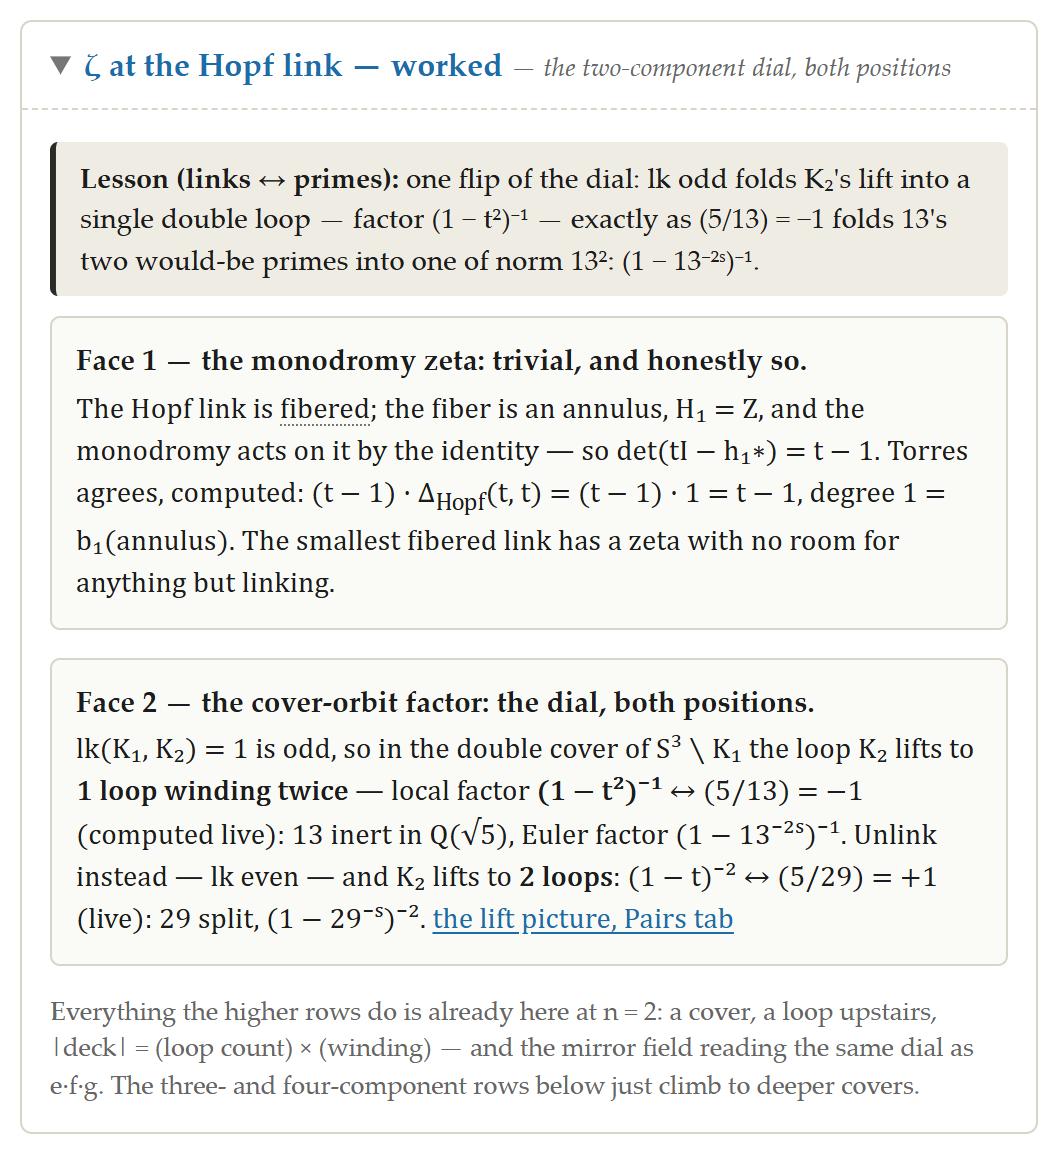
\includegraphics[width=\linewidth]{img/24-hopf-card.png}
\column{0.33\textwidth}\centering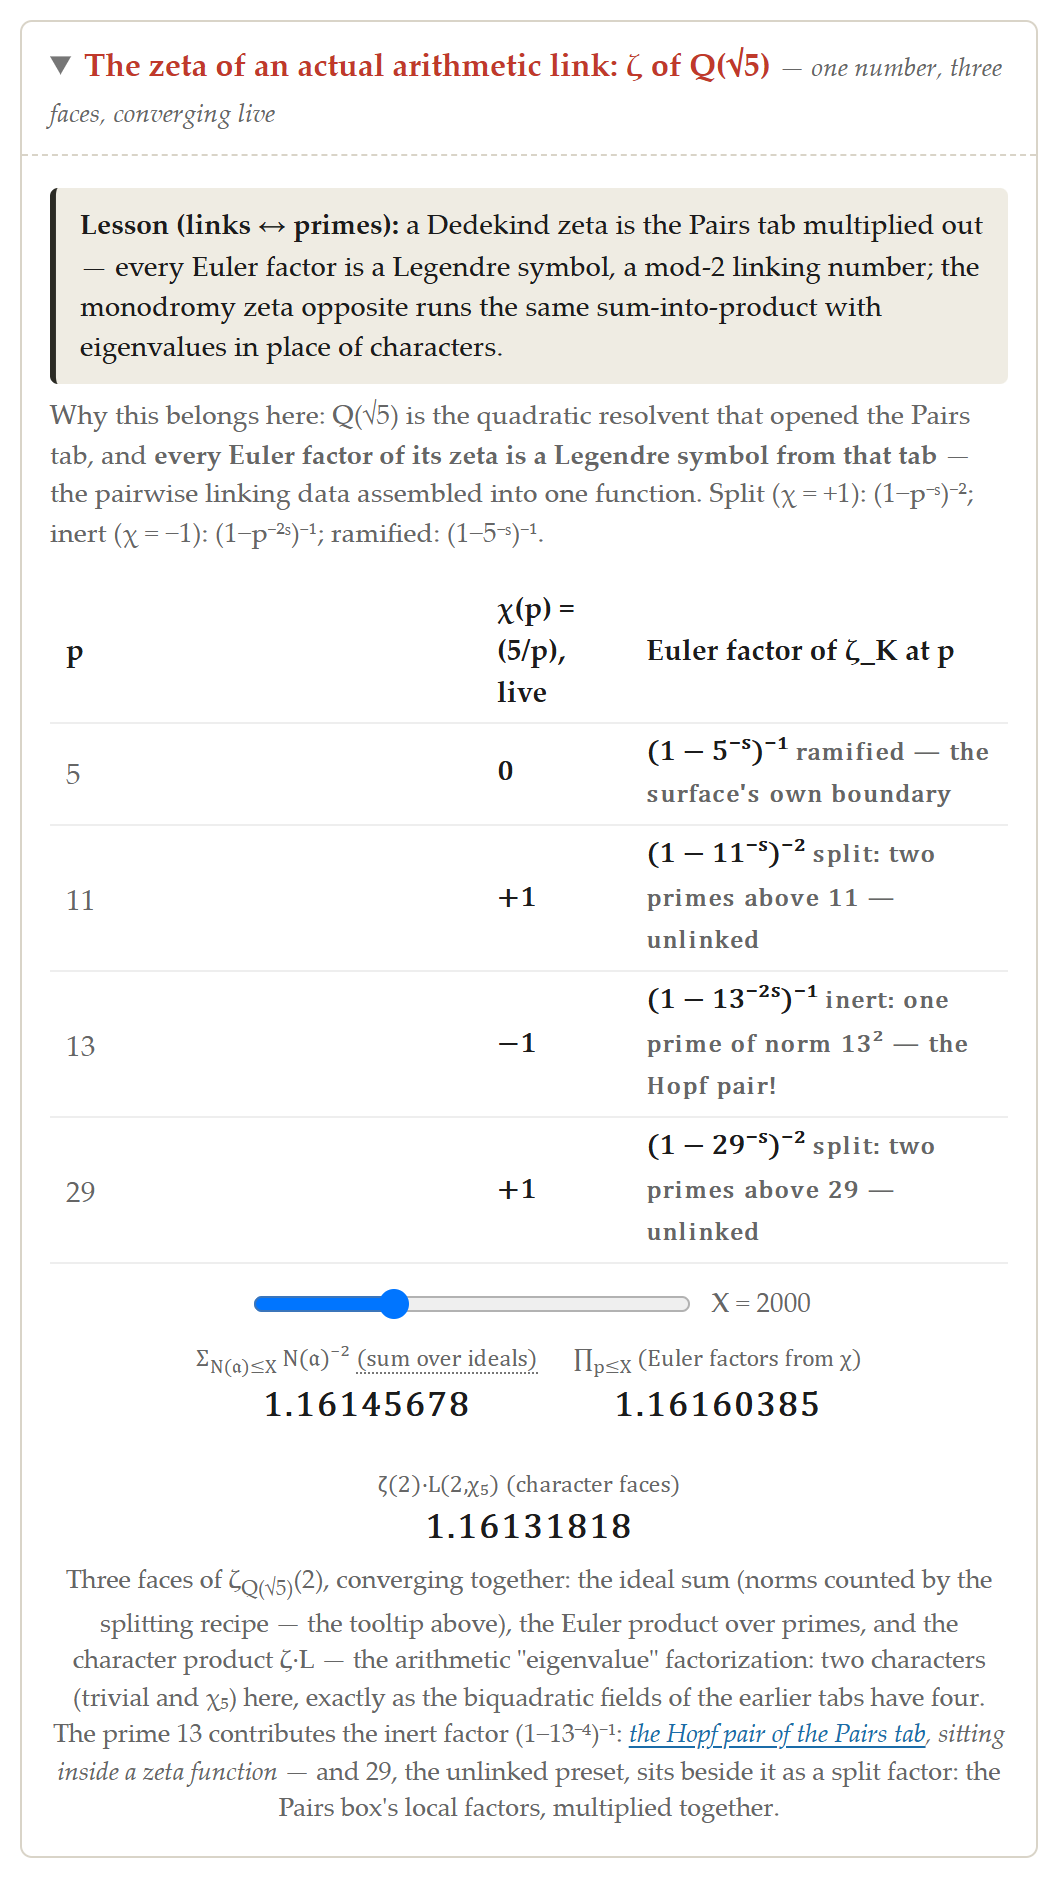
\includegraphics[width=\linewidth,trim=0 929 0 0,clip]{img/25-sqrt5-card.png}
\column{0.33\textwidth}\centering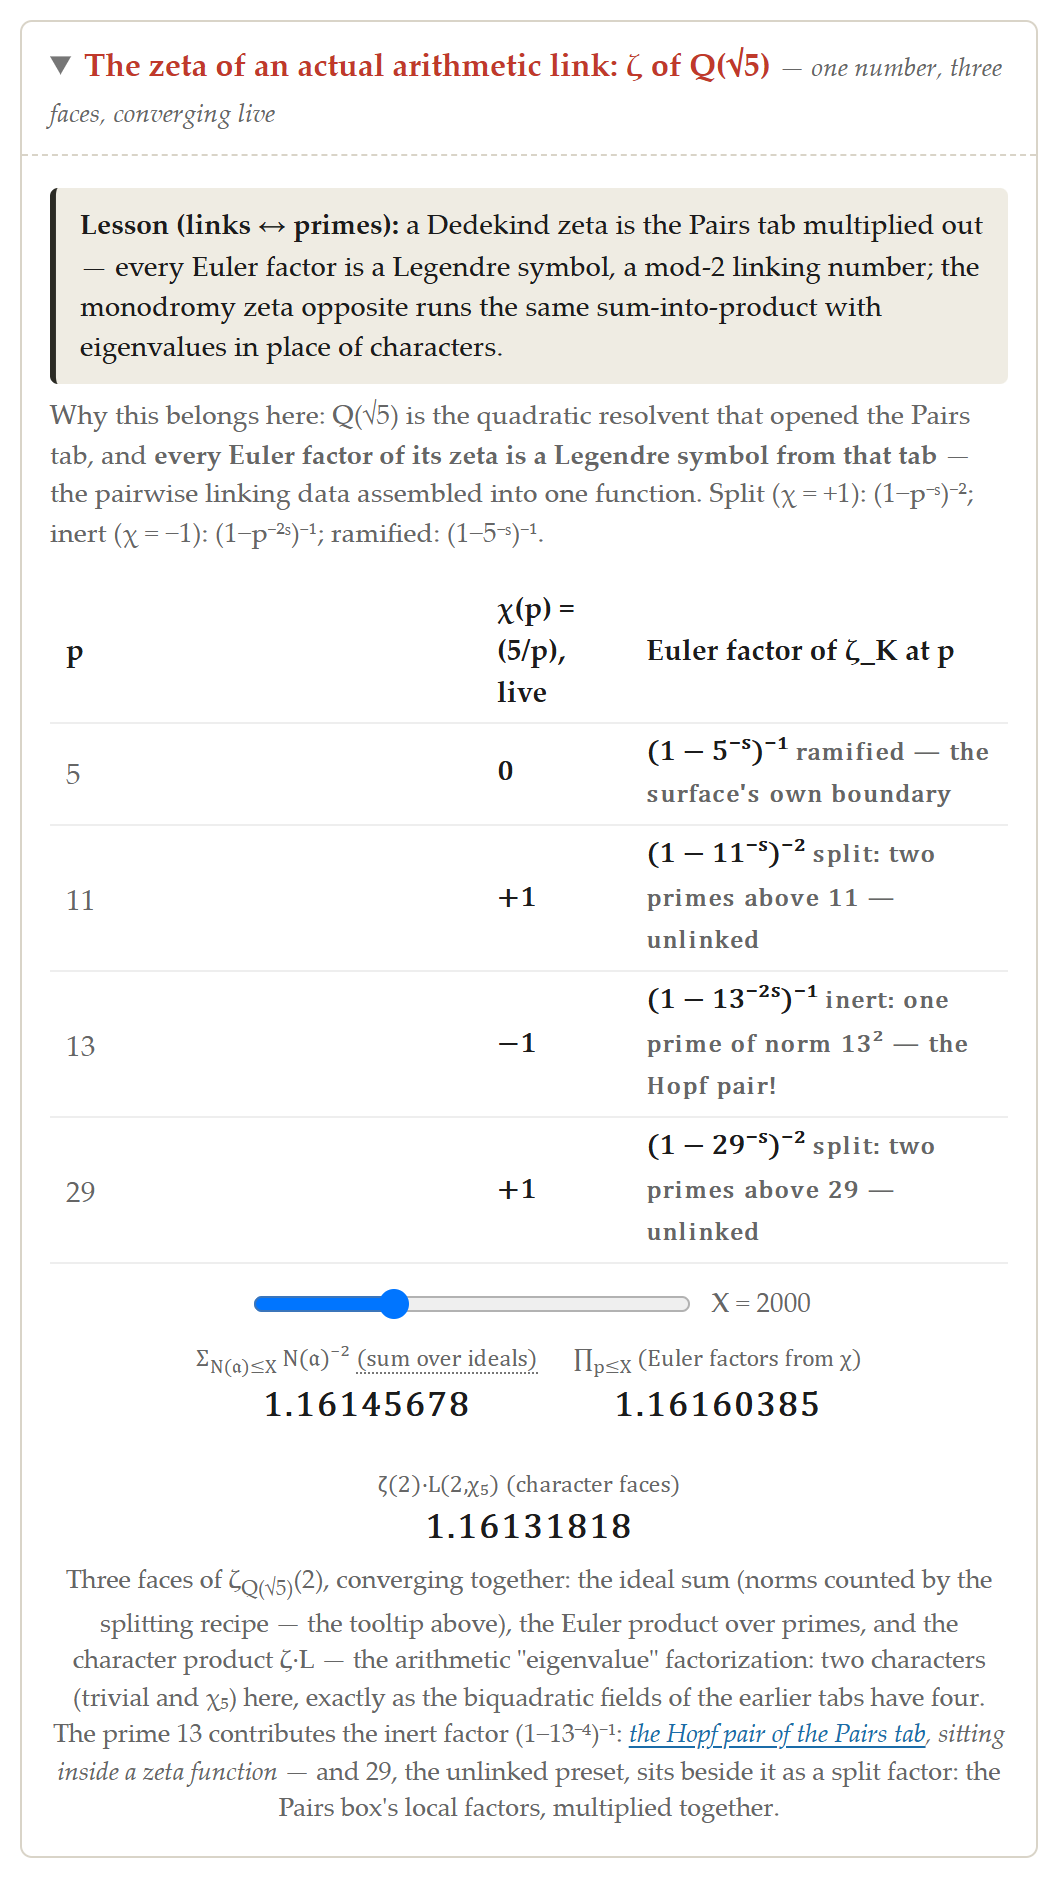
\includegraphics[width=\linewidth,trim=0 0 0 929,clip]{img/25-sqrt5-card.png}
\end{columns}
\vspace{2pt}
{\scriptsize\St{Hopf: annulus fiber, monodromy zeta $t-1$, and the dial in both positions --- $(1-t^2)^{-1}\leftrightarrow 13$ inert, $(1-t)^{-2}\leftrightarrow 29$ split. Beside it (card in two panels), $\zeta_{\mathbb{Q}(\sqrt5)}(2)$ computed three ways, converging live on the slider.}}
\end{frame}

% ---------------------------------------------------------------- 21 three components worked (k1361)
\begin{frame}{Three components, worked --- the Borromean field}
\begin{columns}[T]
\column{0.32\textwidth}\centering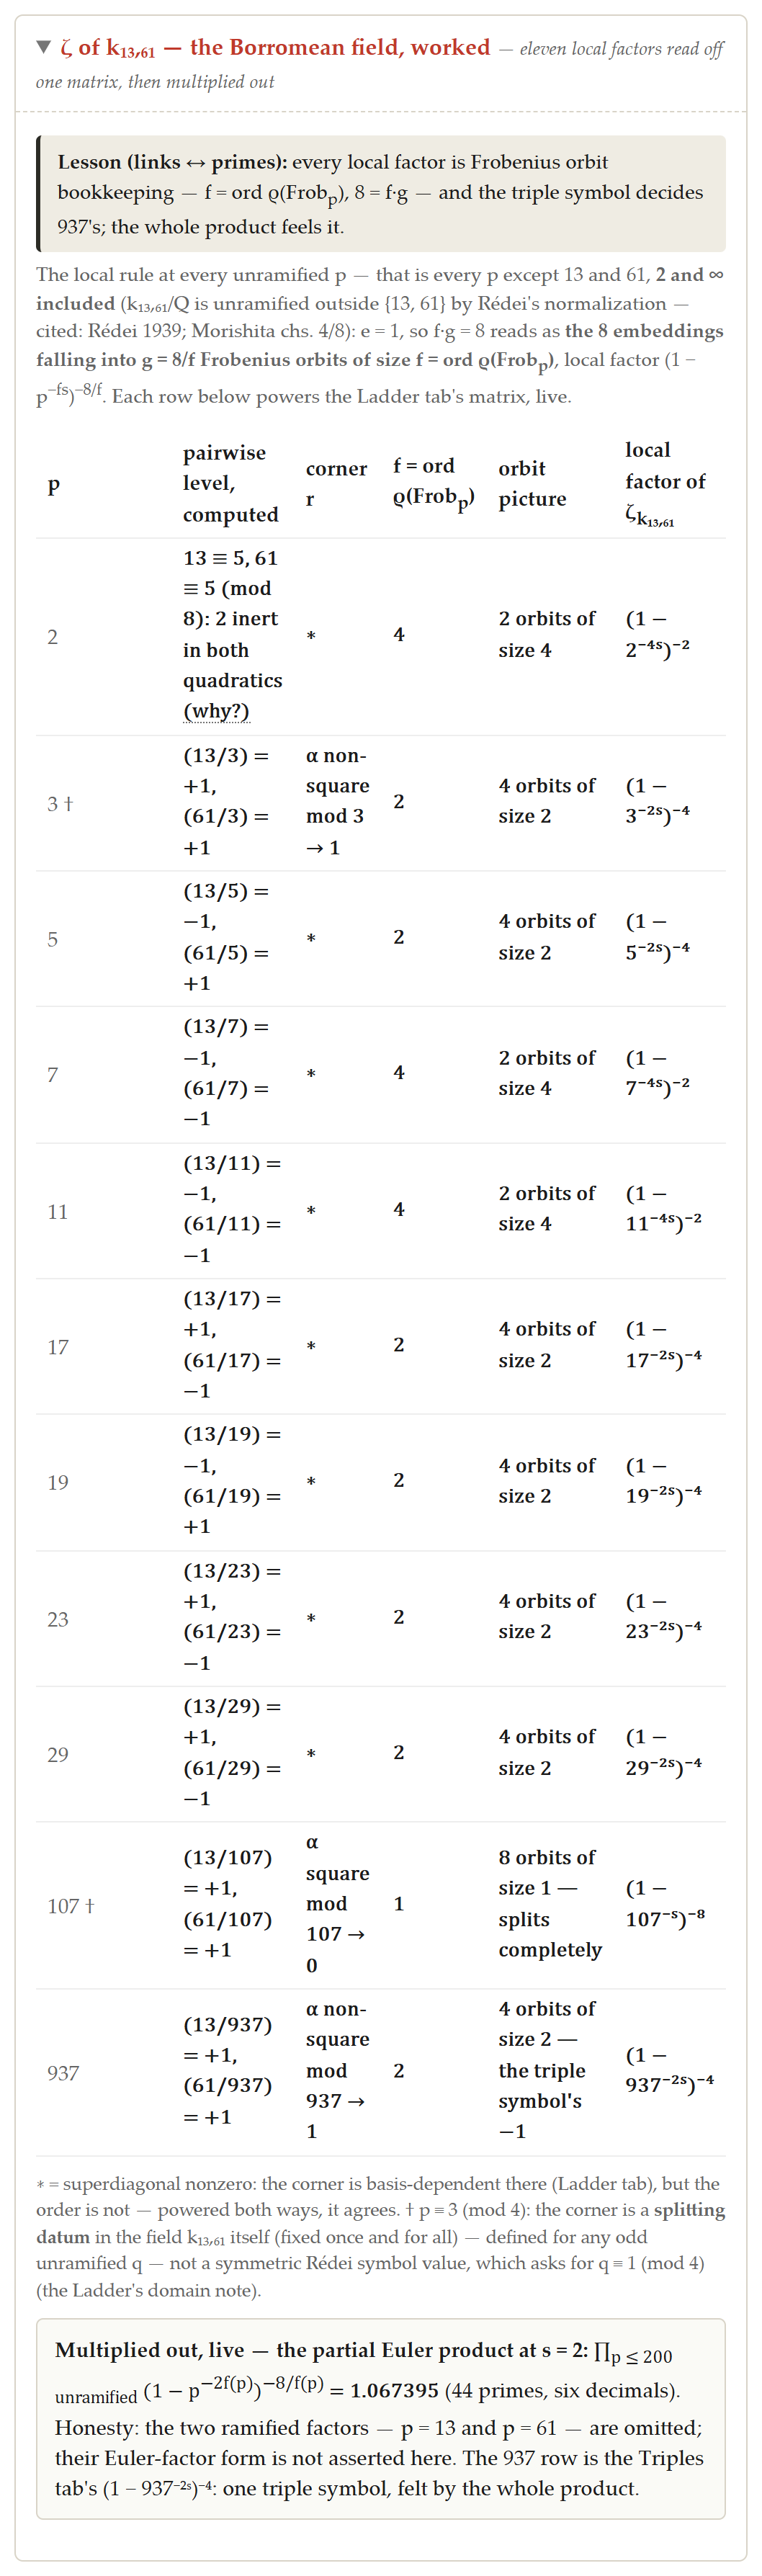
\includegraphics[width=\linewidth,trim=0 2384 0 0,clip]{img/26-k1361-card.png}
\column{0.32\textwidth}\centering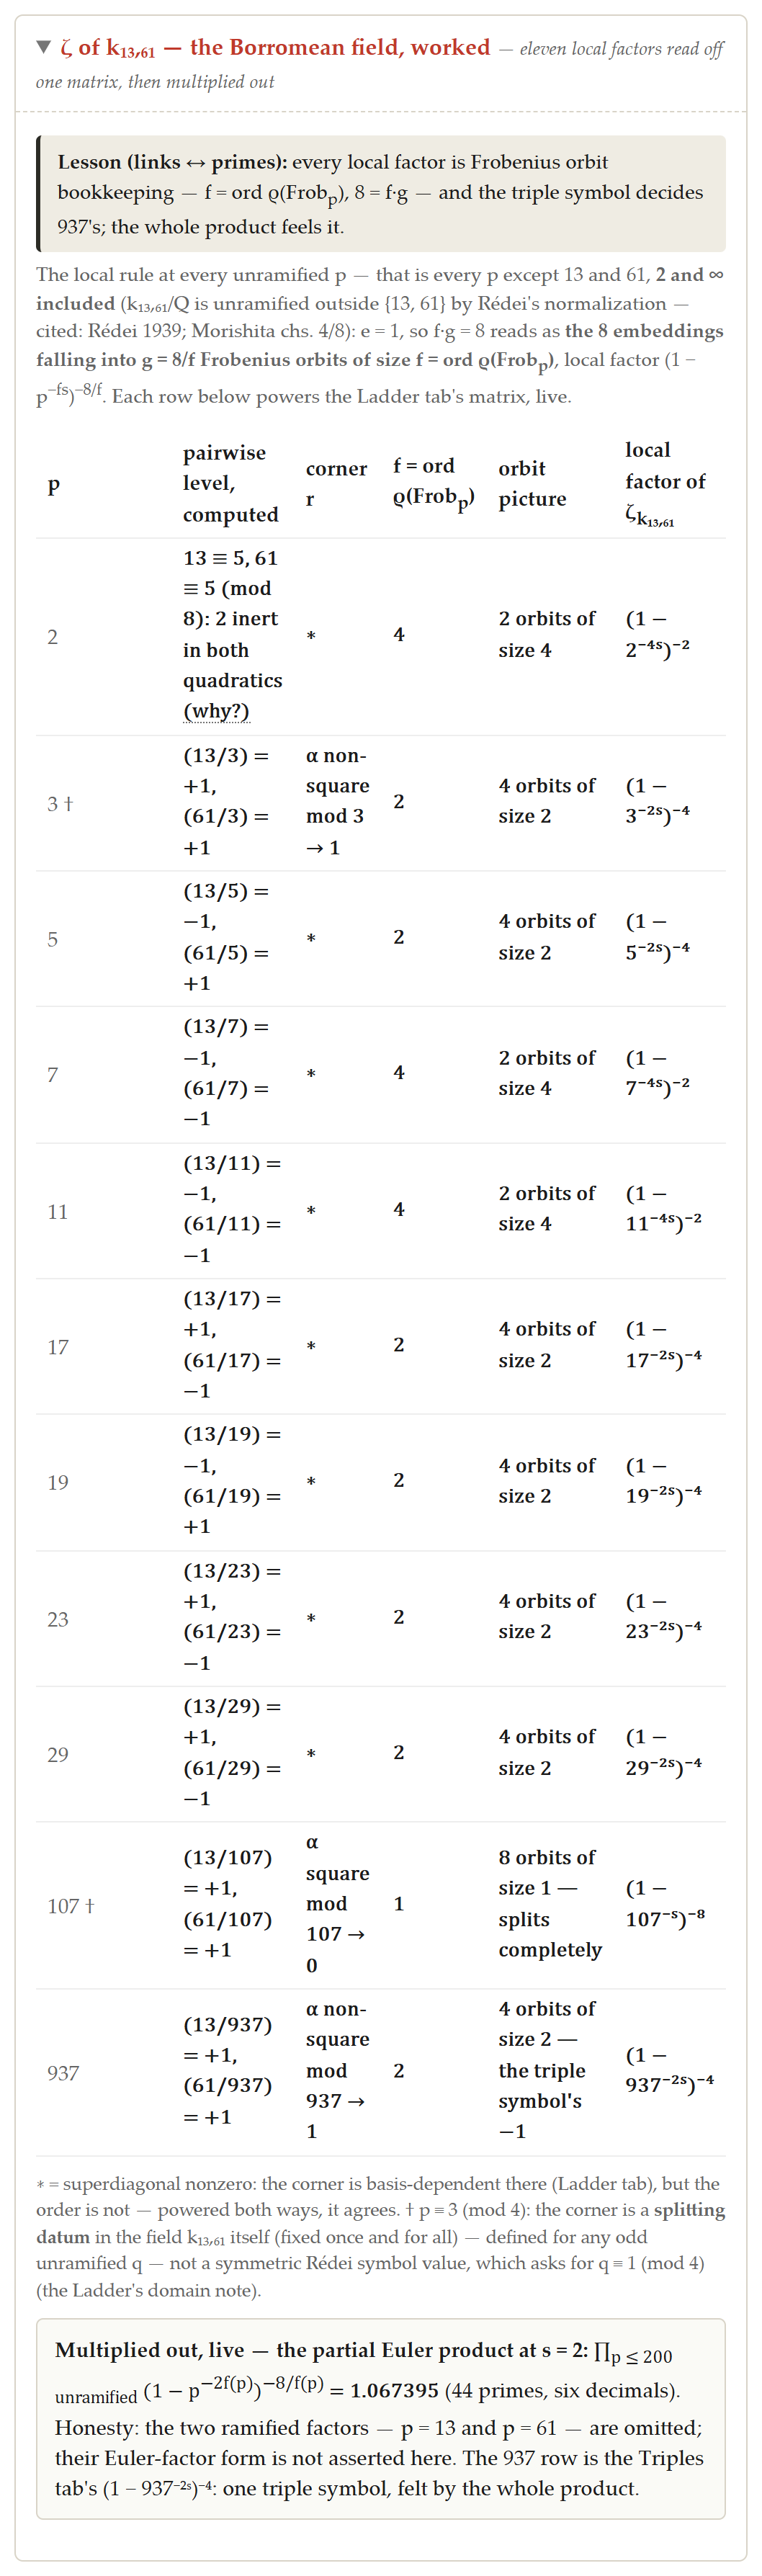
\includegraphics[width=\linewidth,trim=0 1192 0 1192,clip]{img/26-k1361-card.png}
\column{0.32\textwidth}\centering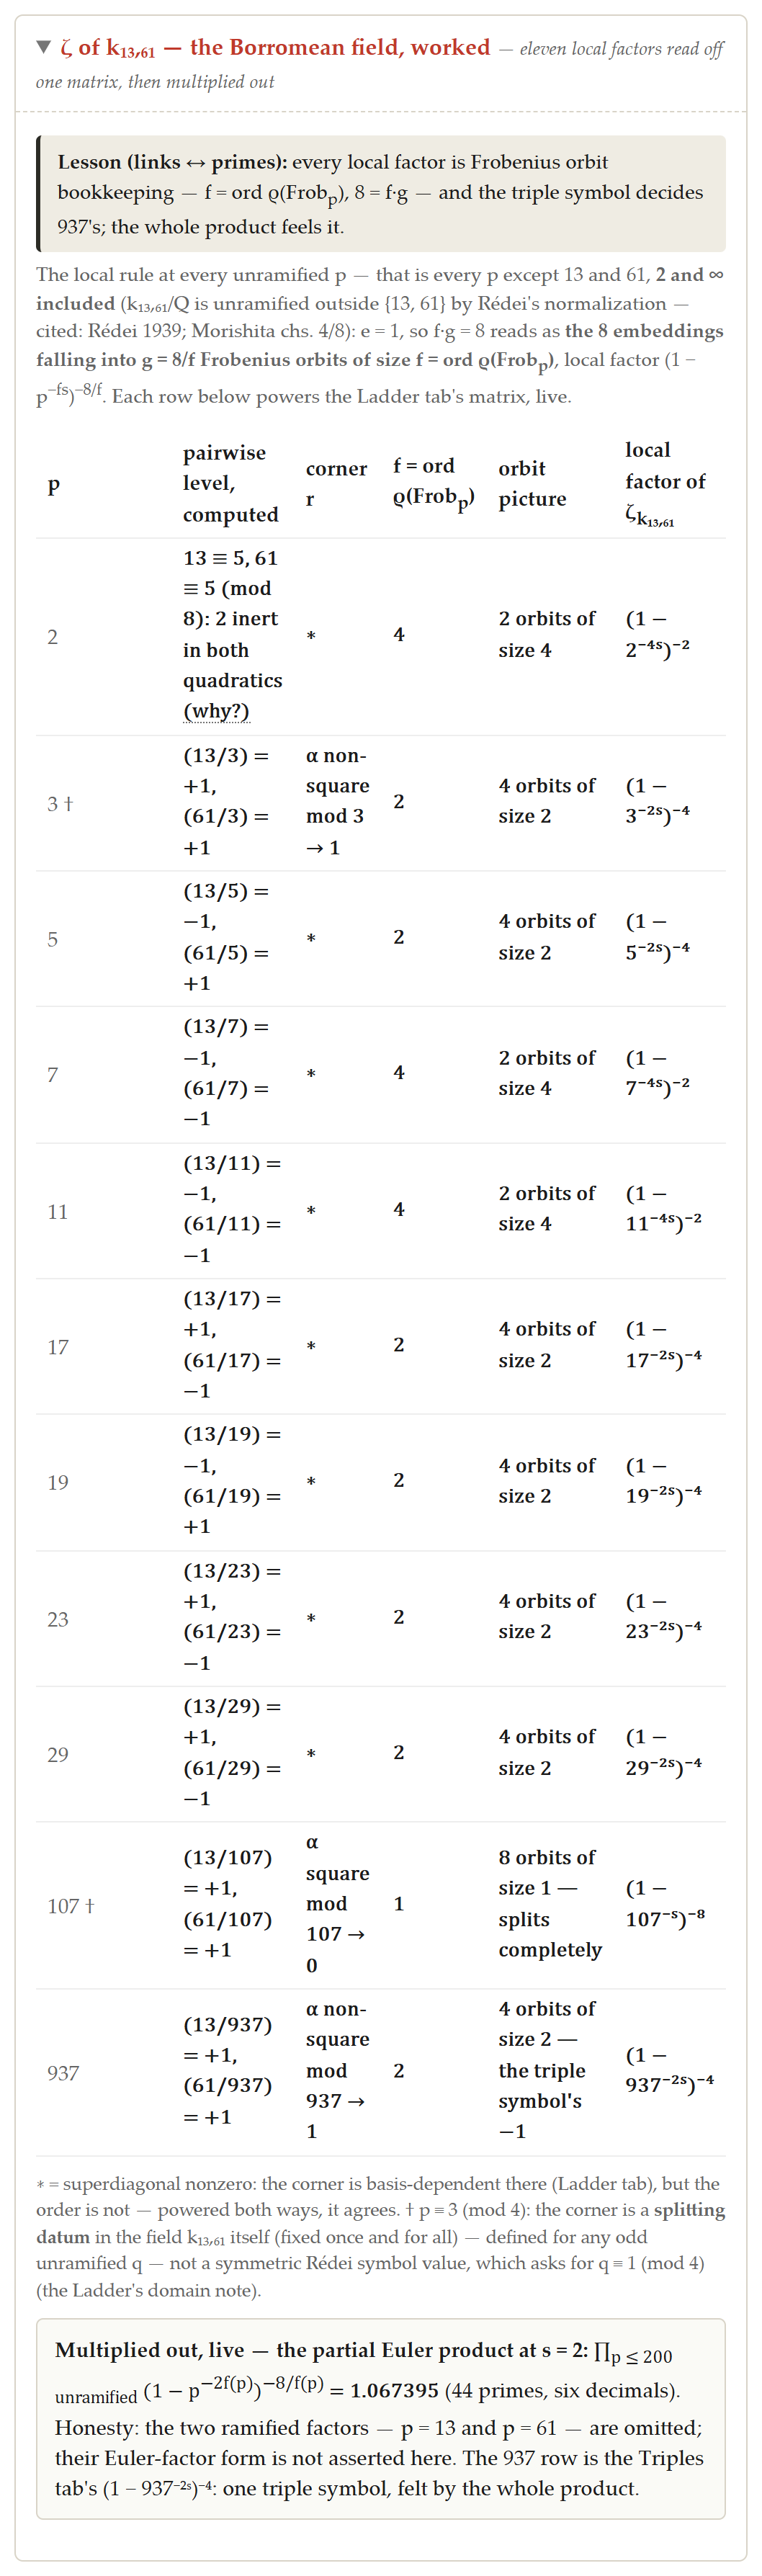
\includegraphics[width=\linewidth,trim=0 0 0 2384,clip]{img/26-k1361-card.png}
\end{columns}
\vspace{2pt}
{\scriptsize\St{One card, three panels: eleven local factors of $\zeta_{k_{13,61}}$ read off matrix orders --- 107 splits completely, 937 carries the triple symbol's $-1$ --- multiplied out at $s=2$: $\mathbf{1.067395}$ over the 44 unramified $p\le200$, ramified factors omitted and said so.}}
\end{frame}

% ---------------------------------------------------------------- 21b borromean worked
\begin{frame}{Three components, worked --- the link's two zetas}
\begin{columns}[T]
\column{0.62\textwidth}\shot[0.66\textheight]{img/27-borro-worked.png}
\column{0.36\textwidth}
{\scriptsize\St{Kept visibly distinct: the monodromy zeta --- $\exp(\sum 4t^n/n)=(1-t)^{-4}$, checked coefficient by coefficient, $1,4,10,20,35,\dots$ --- and the cover-orbit factor $(1-t^2)^{-4}$: 4 loops winding twice among the 8 sheets, the exact twin of 937's Euler factor.}}
\medskip
\kleinnote{Math: the six-decimal Euler product on the previous slide is the strongest single exhibit in the talk --- an actual degree-8 Dedekind zeta, worked. Keep it late, as here.}
\end{columns}
\end{frame}

% ---------------------------------------------------------------- 22 four components worked
\begin{frame}{Four components, worked}
\begin{columns}[T]
\column{0.32\textwidth}\centering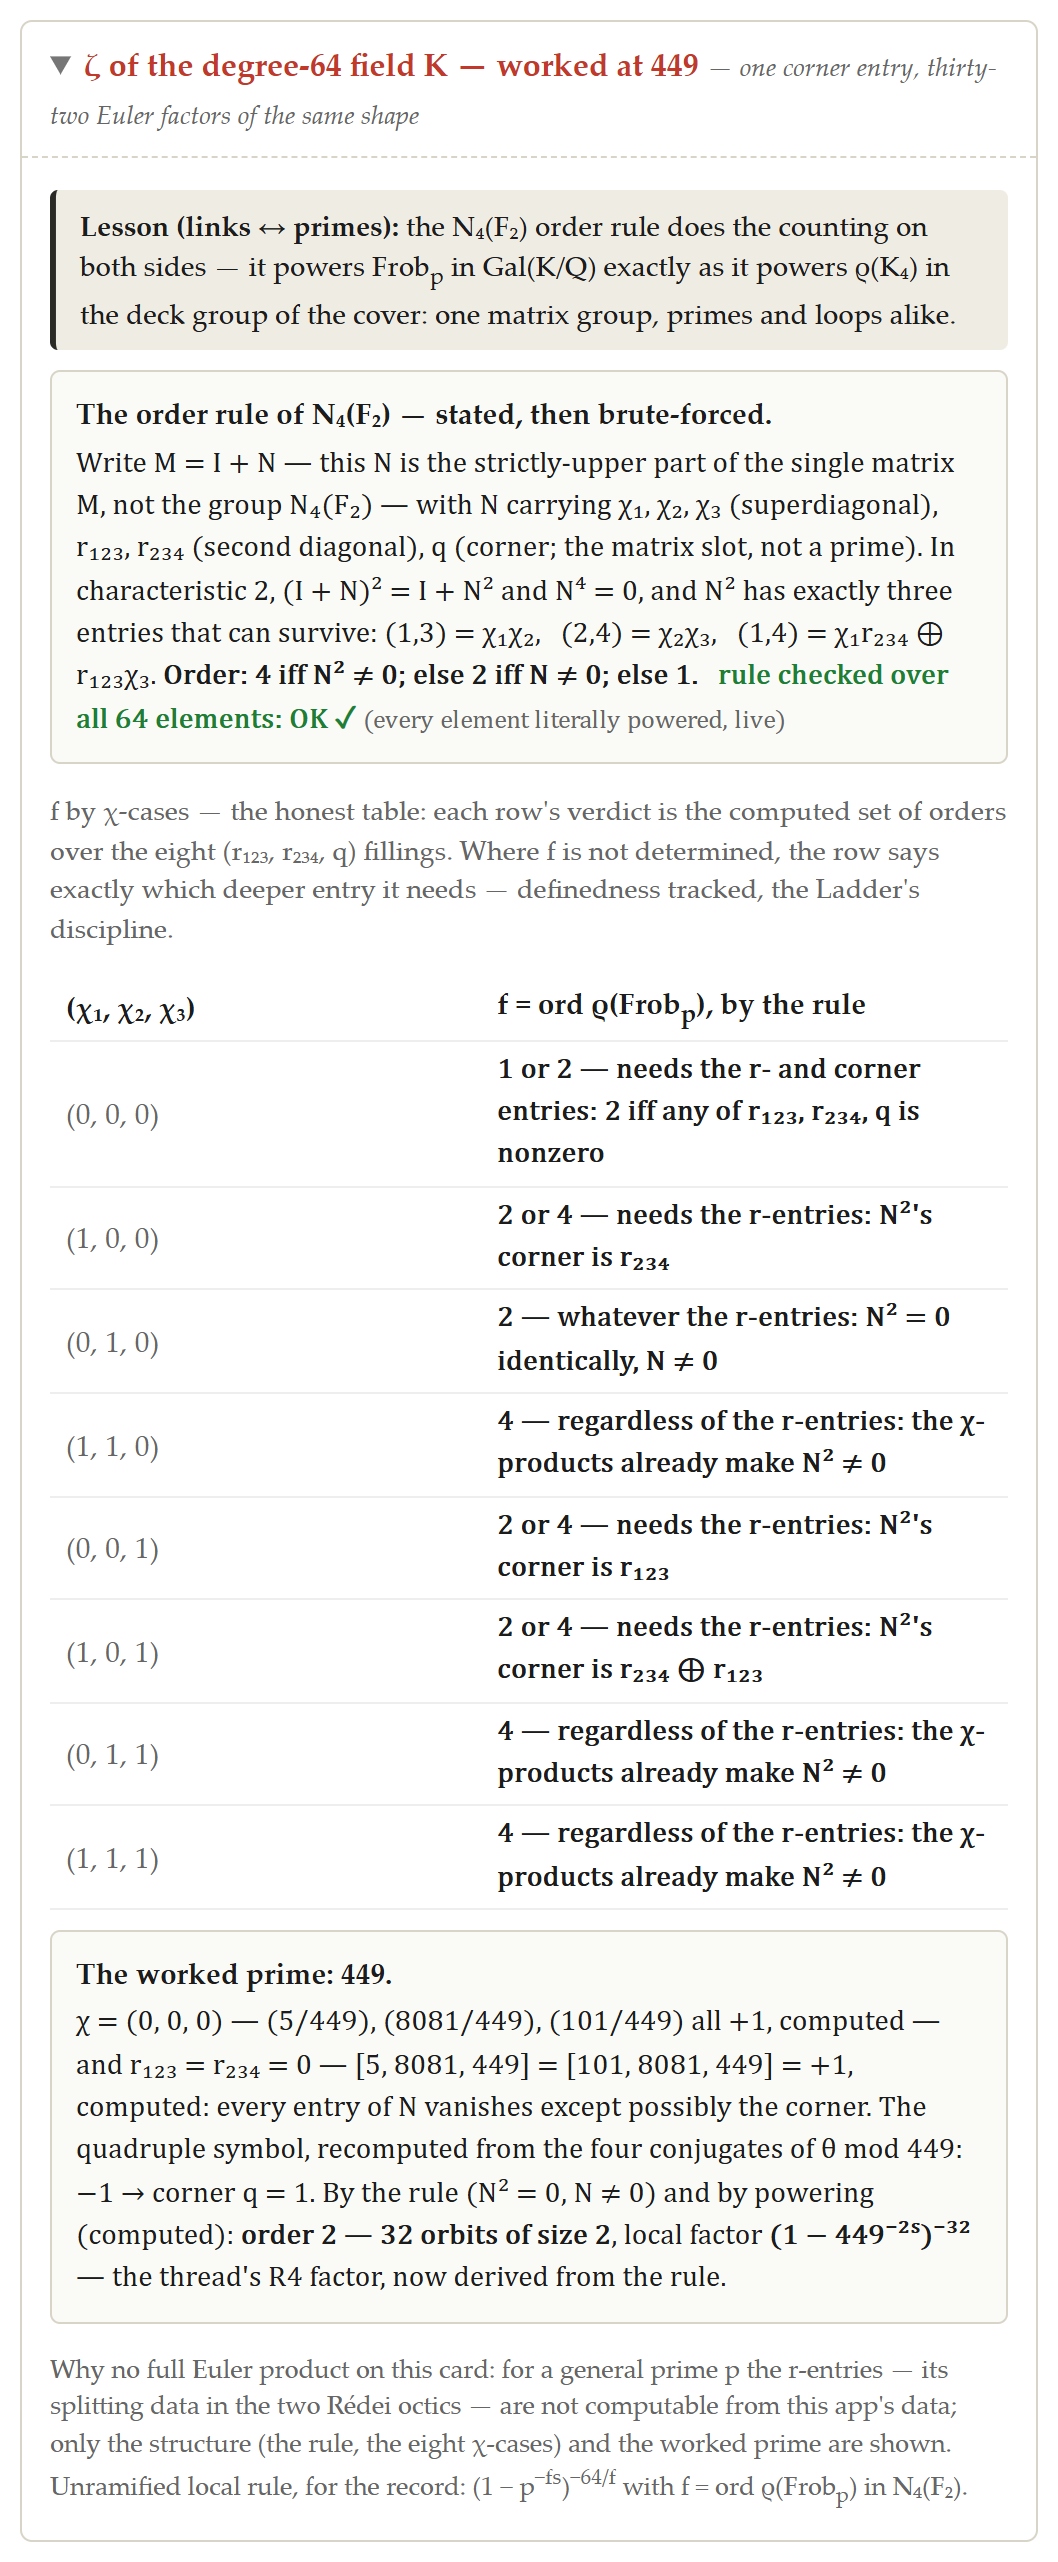
\includegraphics[width=\linewidth,trim=0 1271 0 0,clip]{img/28-449-card.png}
\column{0.32\textwidth}\centering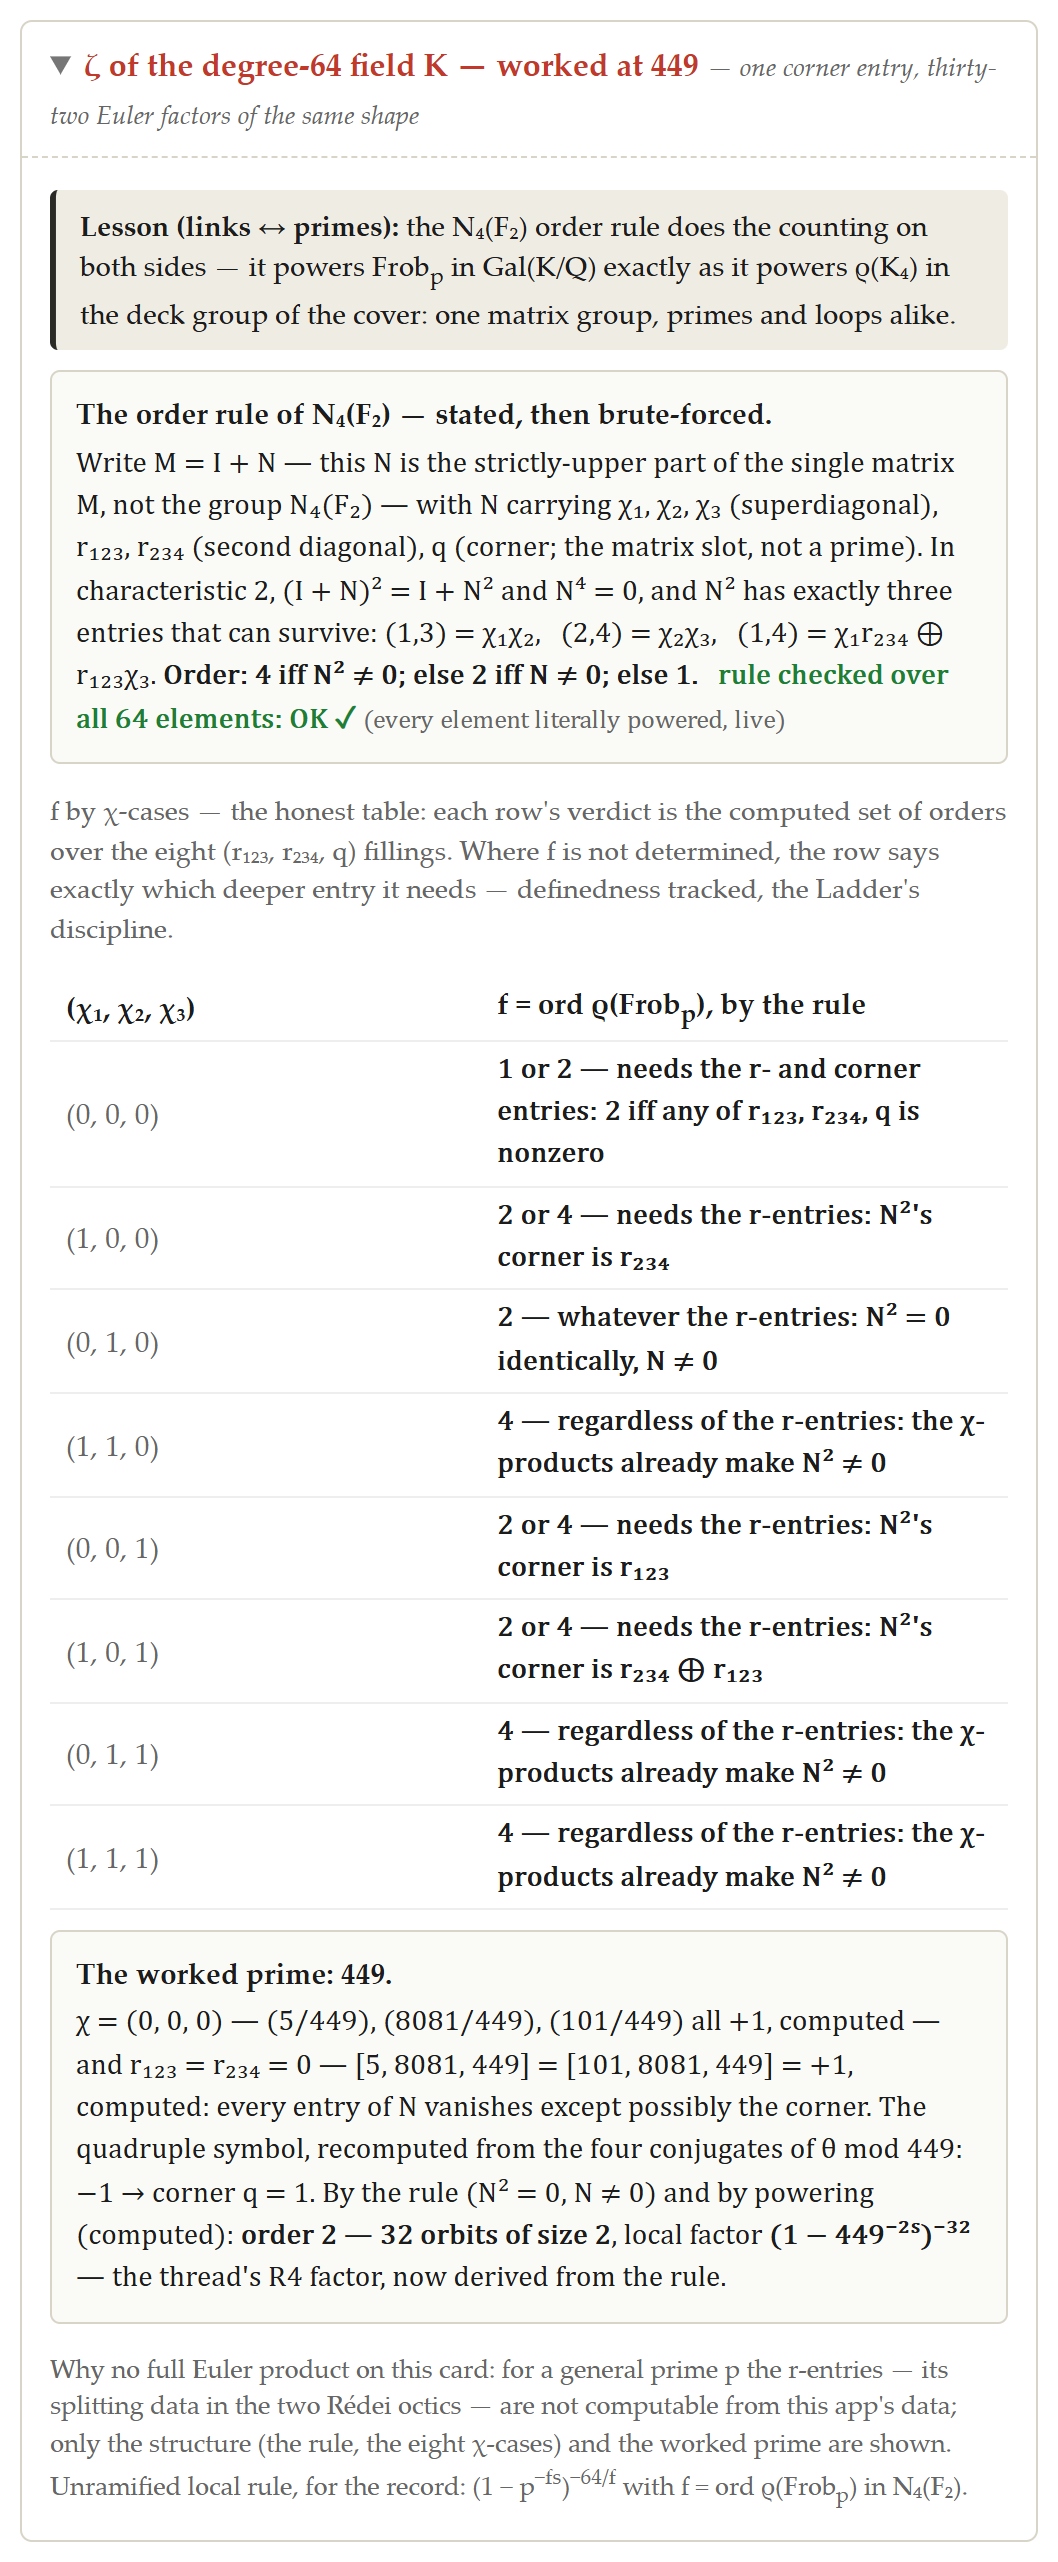
\includegraphics[width=\linewidth,trim=0 0 0 1271,clip]{img/28-449-card.png}
\column{0.32\textwidth}\centering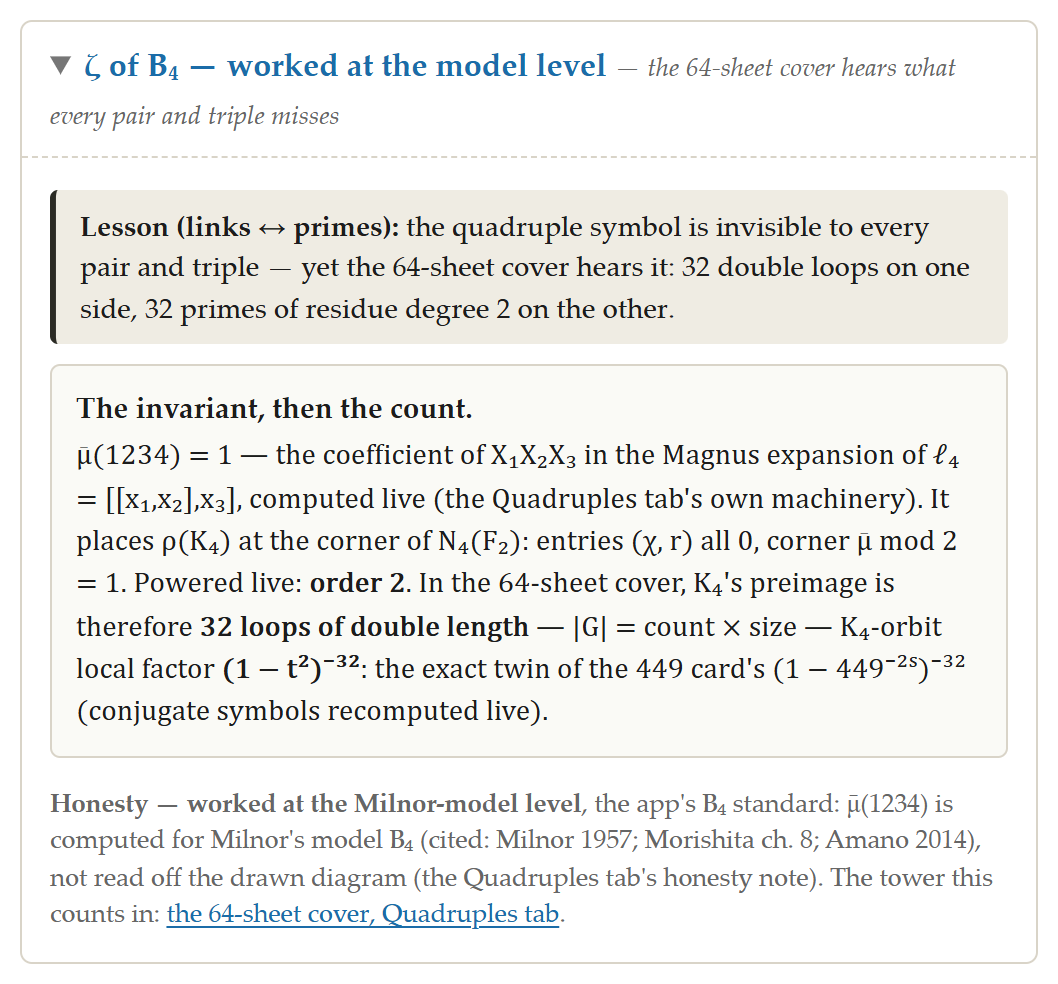
\includegraphics[width=\linewidth]{img/29-b4-card.png}
\end{columns}
\vspace{2pt}
{\scriptsize\St{The $N_4(\mathbb{F}_2)$ order rule stated, then \emph{brute-forced over all 64 elements on screen}; the eight $\chi$-cases with honest ``needs the $r$-entries'' rows; 449 worked: order 2, 32 orbits, $(1-449^{-2s})^{-32}$. Right panel: the model-level $B_4$ twin, $(1-t^2)^{-32}$, honesty label attached.}}
\end{frame}

% ---------------------------------------------------------------- 23 contrast: fig8
\begin{frame}{The contrast: what knotting adds}
\begin{columns}[T]
\column{0.48\textwidth}\centering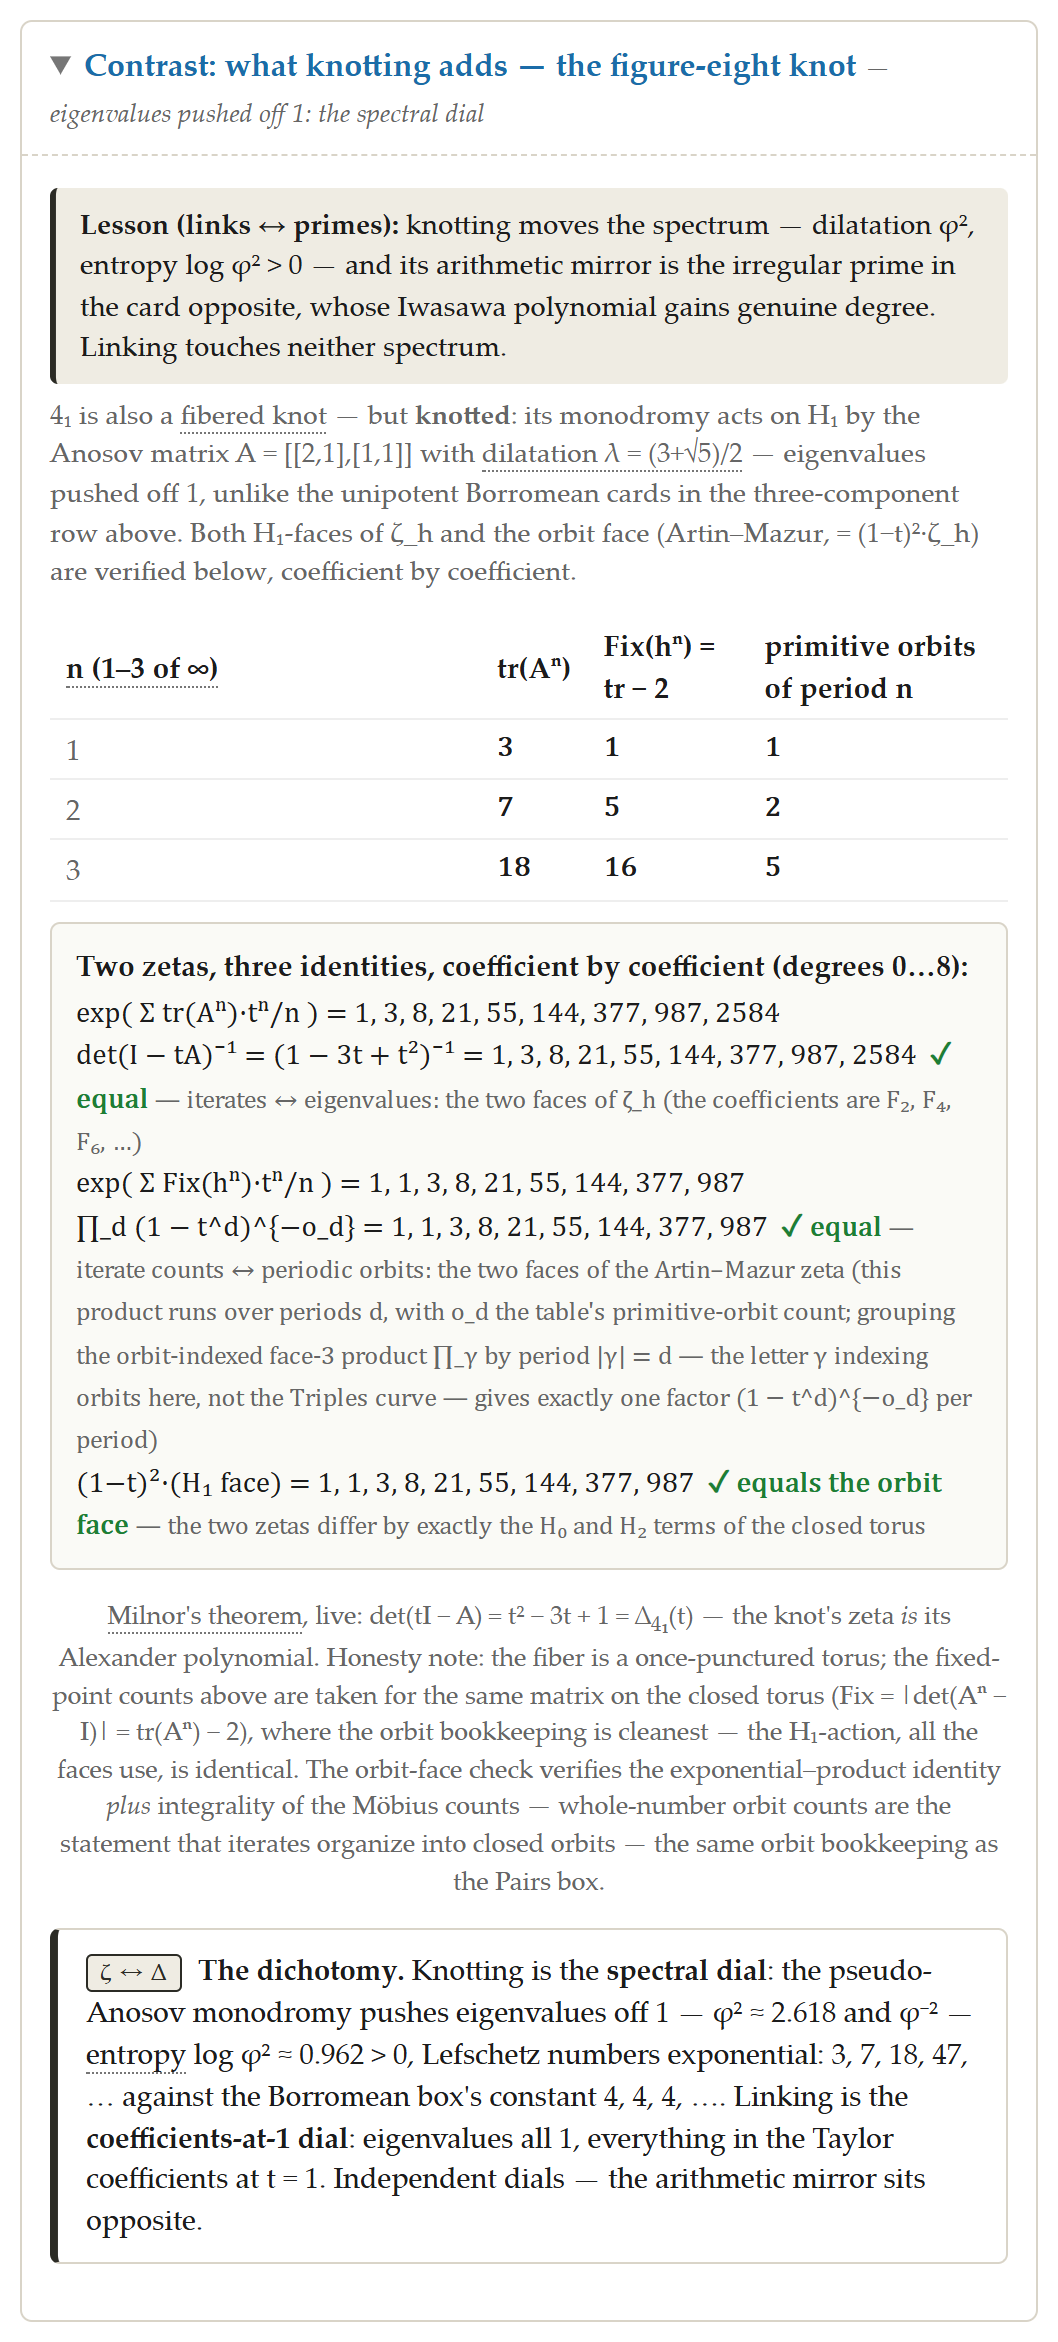
\includegraphics[width=\linewidth,trim=0 1161 0 0,clip]{img/30-fig8-card.png}
\column{0.48\textwidth}\centering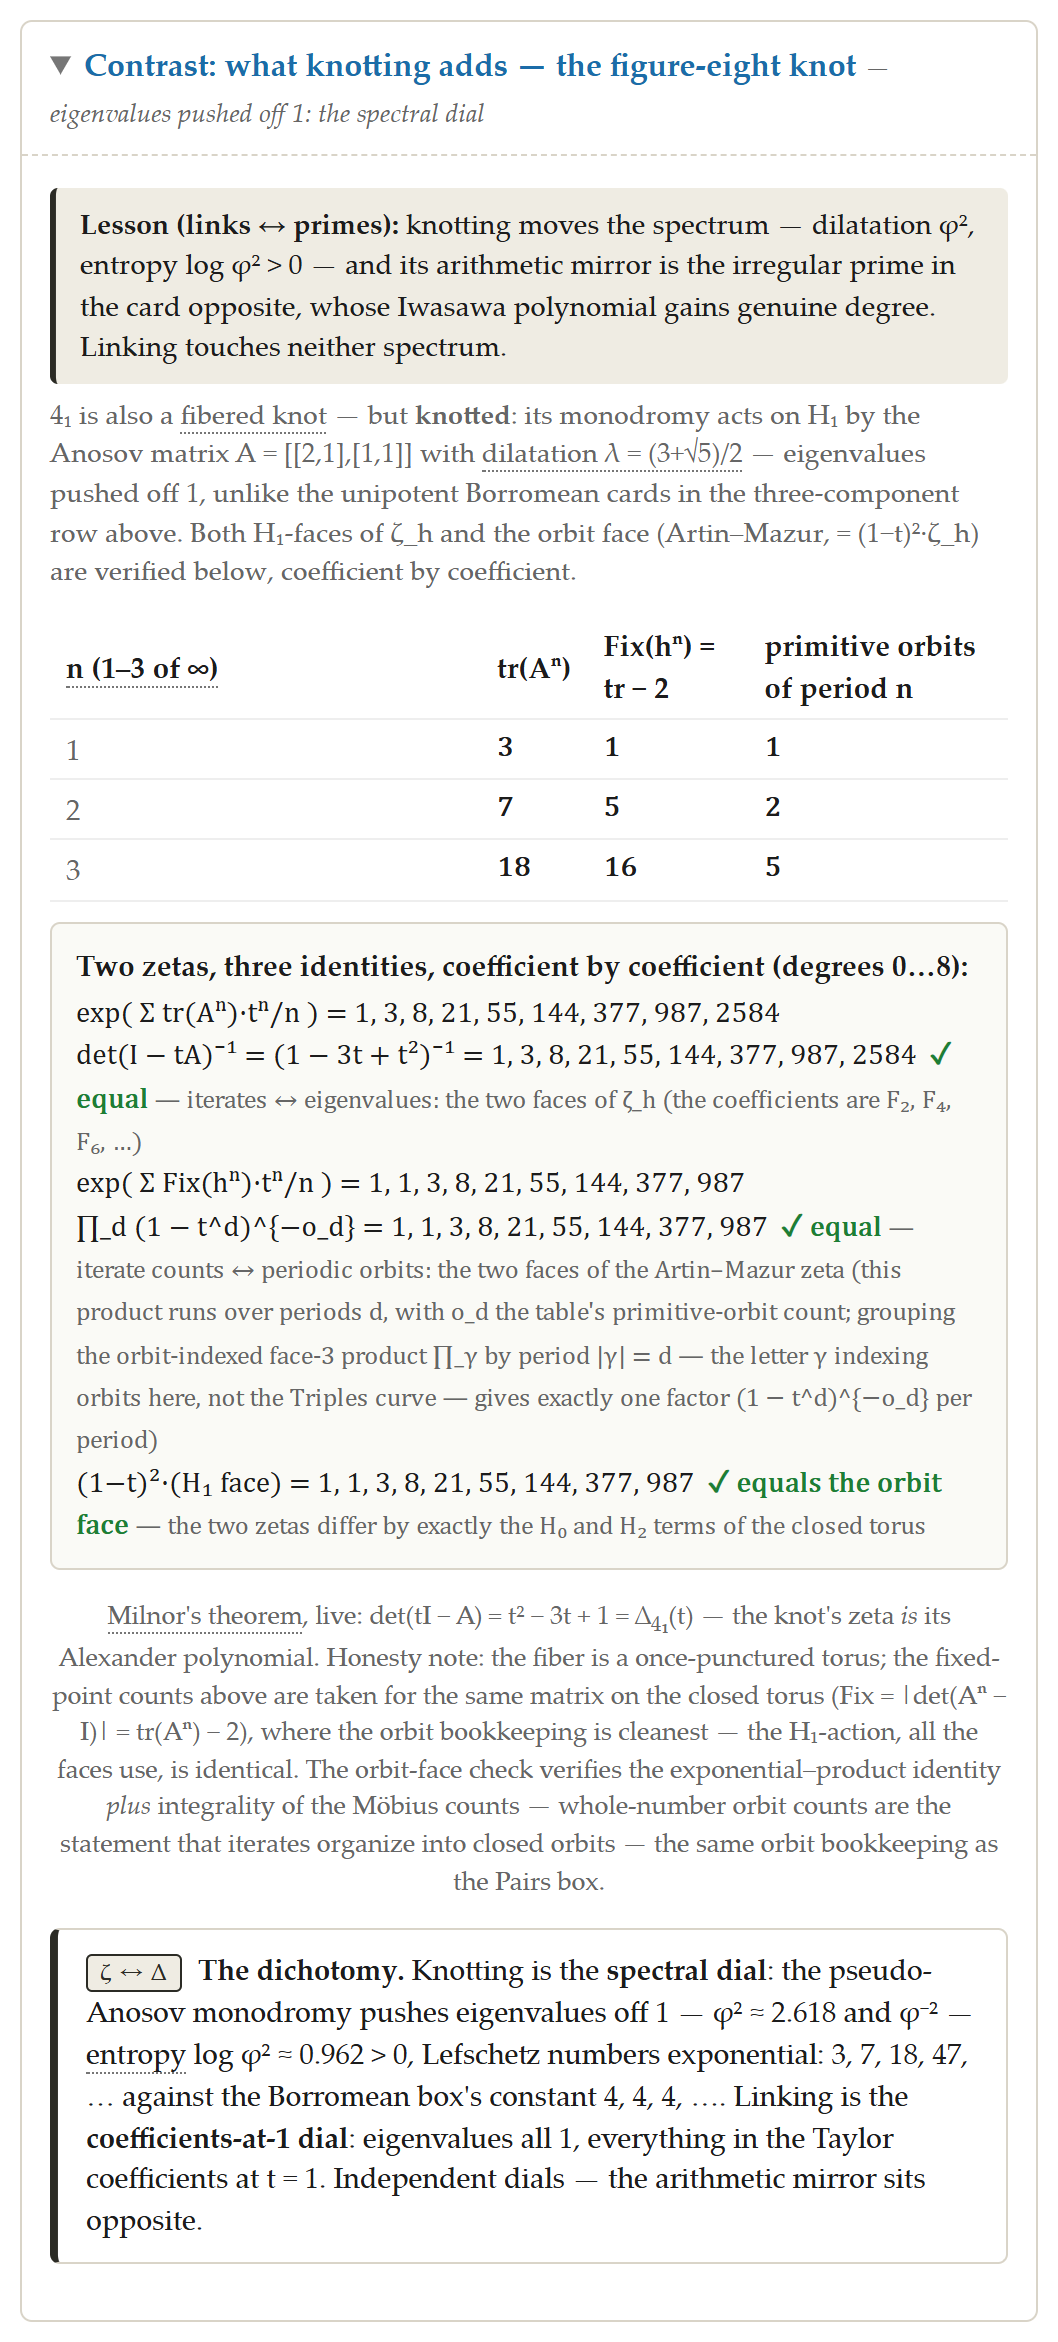
\includegraphics[width=\linewidth,trim=0 0 0 1161,clip]{img/30-fig8-card.png}
\end{columns}
\vspace{2pt}
{\scriptsize\St{Linking lives at $t=1$: unipotent monodromy, Taylor coefficients, the $\bar\mu$ hierarchy. Knotting moves the \emph{spectrum}: the figure-eight's monodromy is Anosov, stretch $\varphi^2$, entropy $\log\varphi^2\approx0.962$, traces $3,7,18,47$ --- all three zeta faces checked coefficient by coefficient in the card.}}
\end{frame}

% ---------------------------------------------------------------- 23b contrast: knotted primes + jewel
\begin{frame}{The knotted primes --- and the jewel}
\begin{columns}[T]
\column{0.48\textwidth}\centering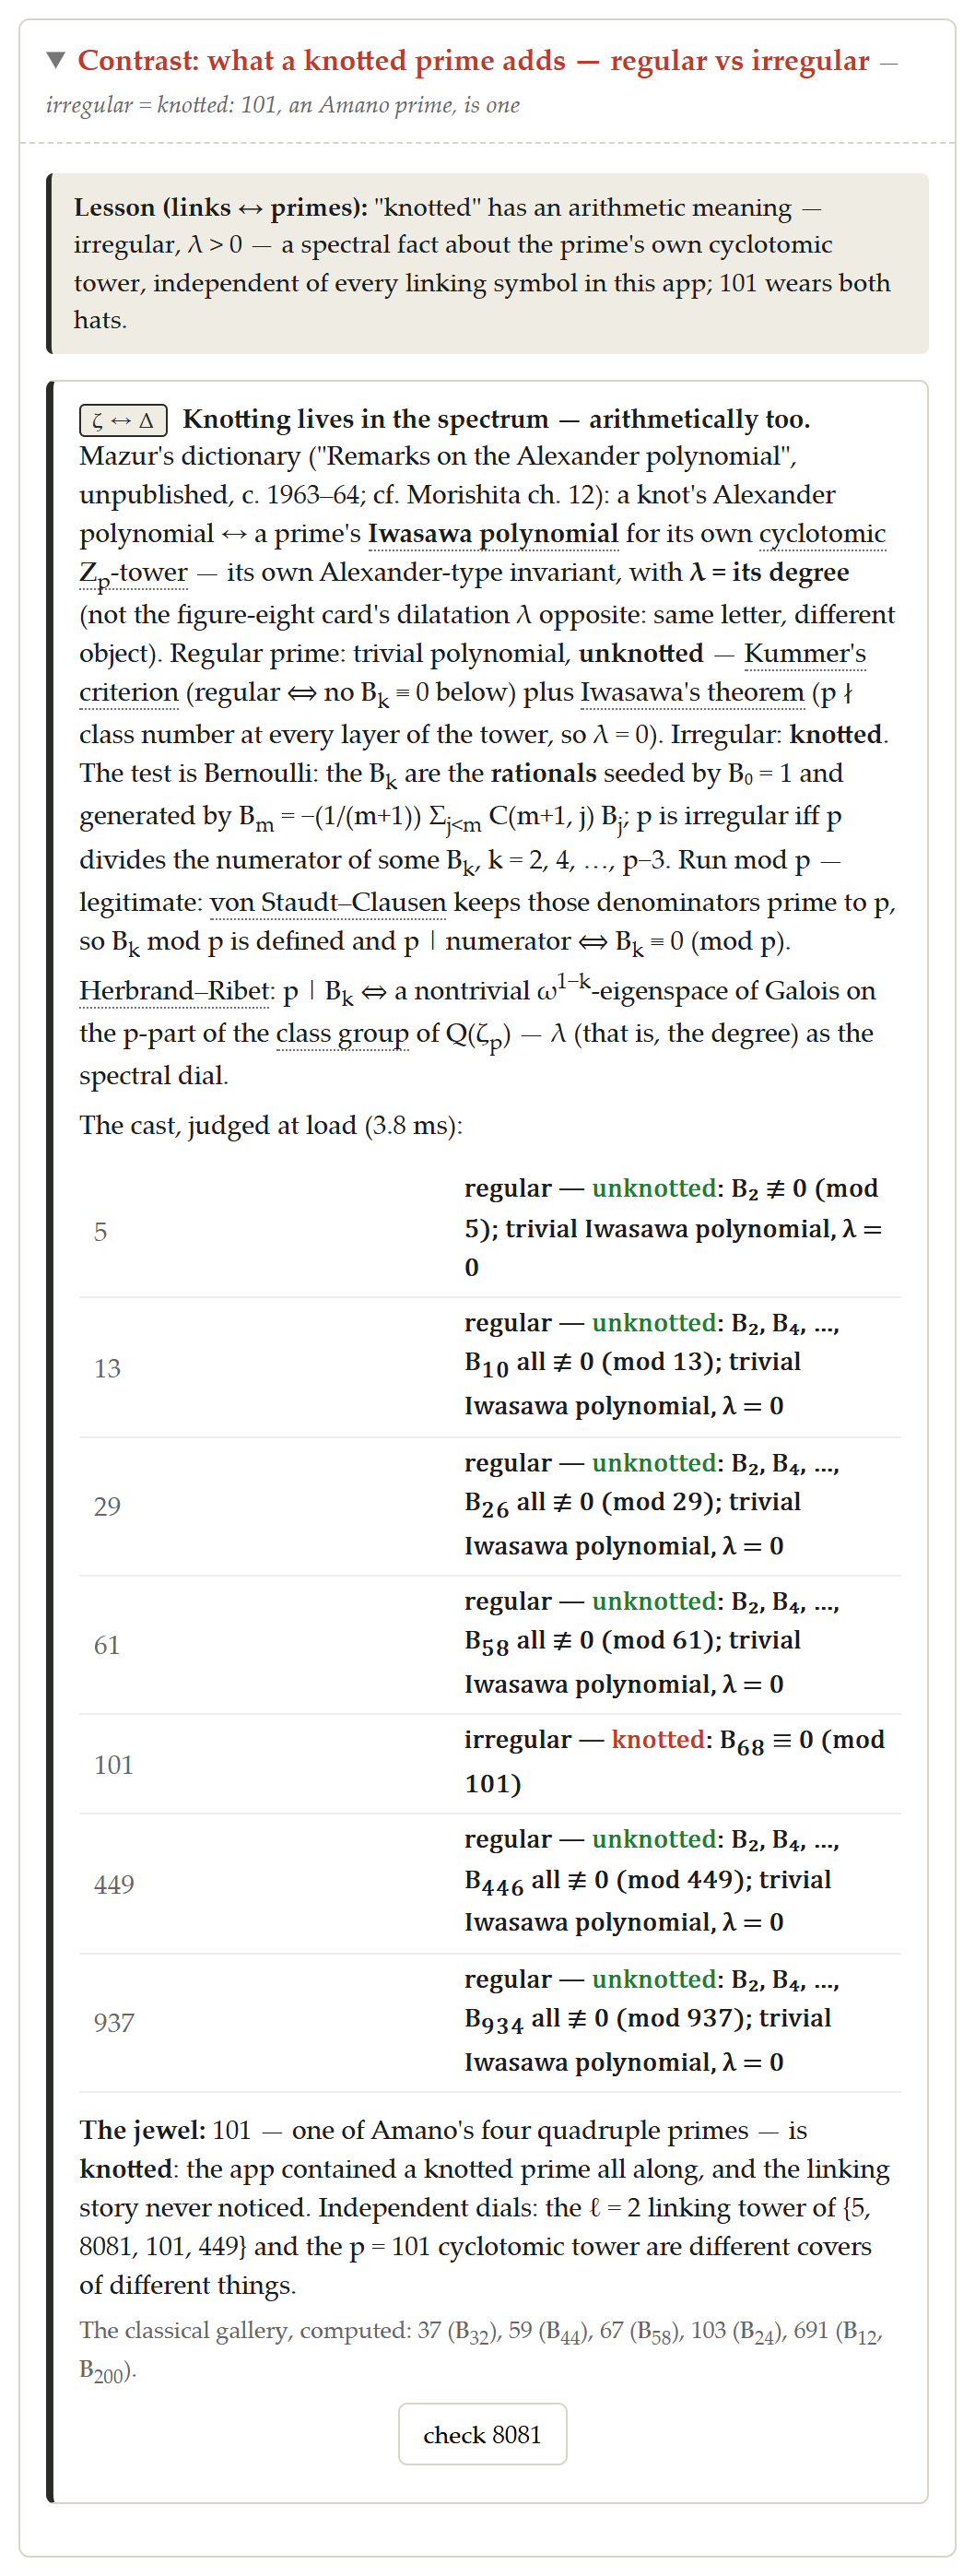
\includegraphics[width=\linewidth,trim=0 1387 0 0,clip]{img/31-knotted-card.png}
\column{0.48\textwidth}\centering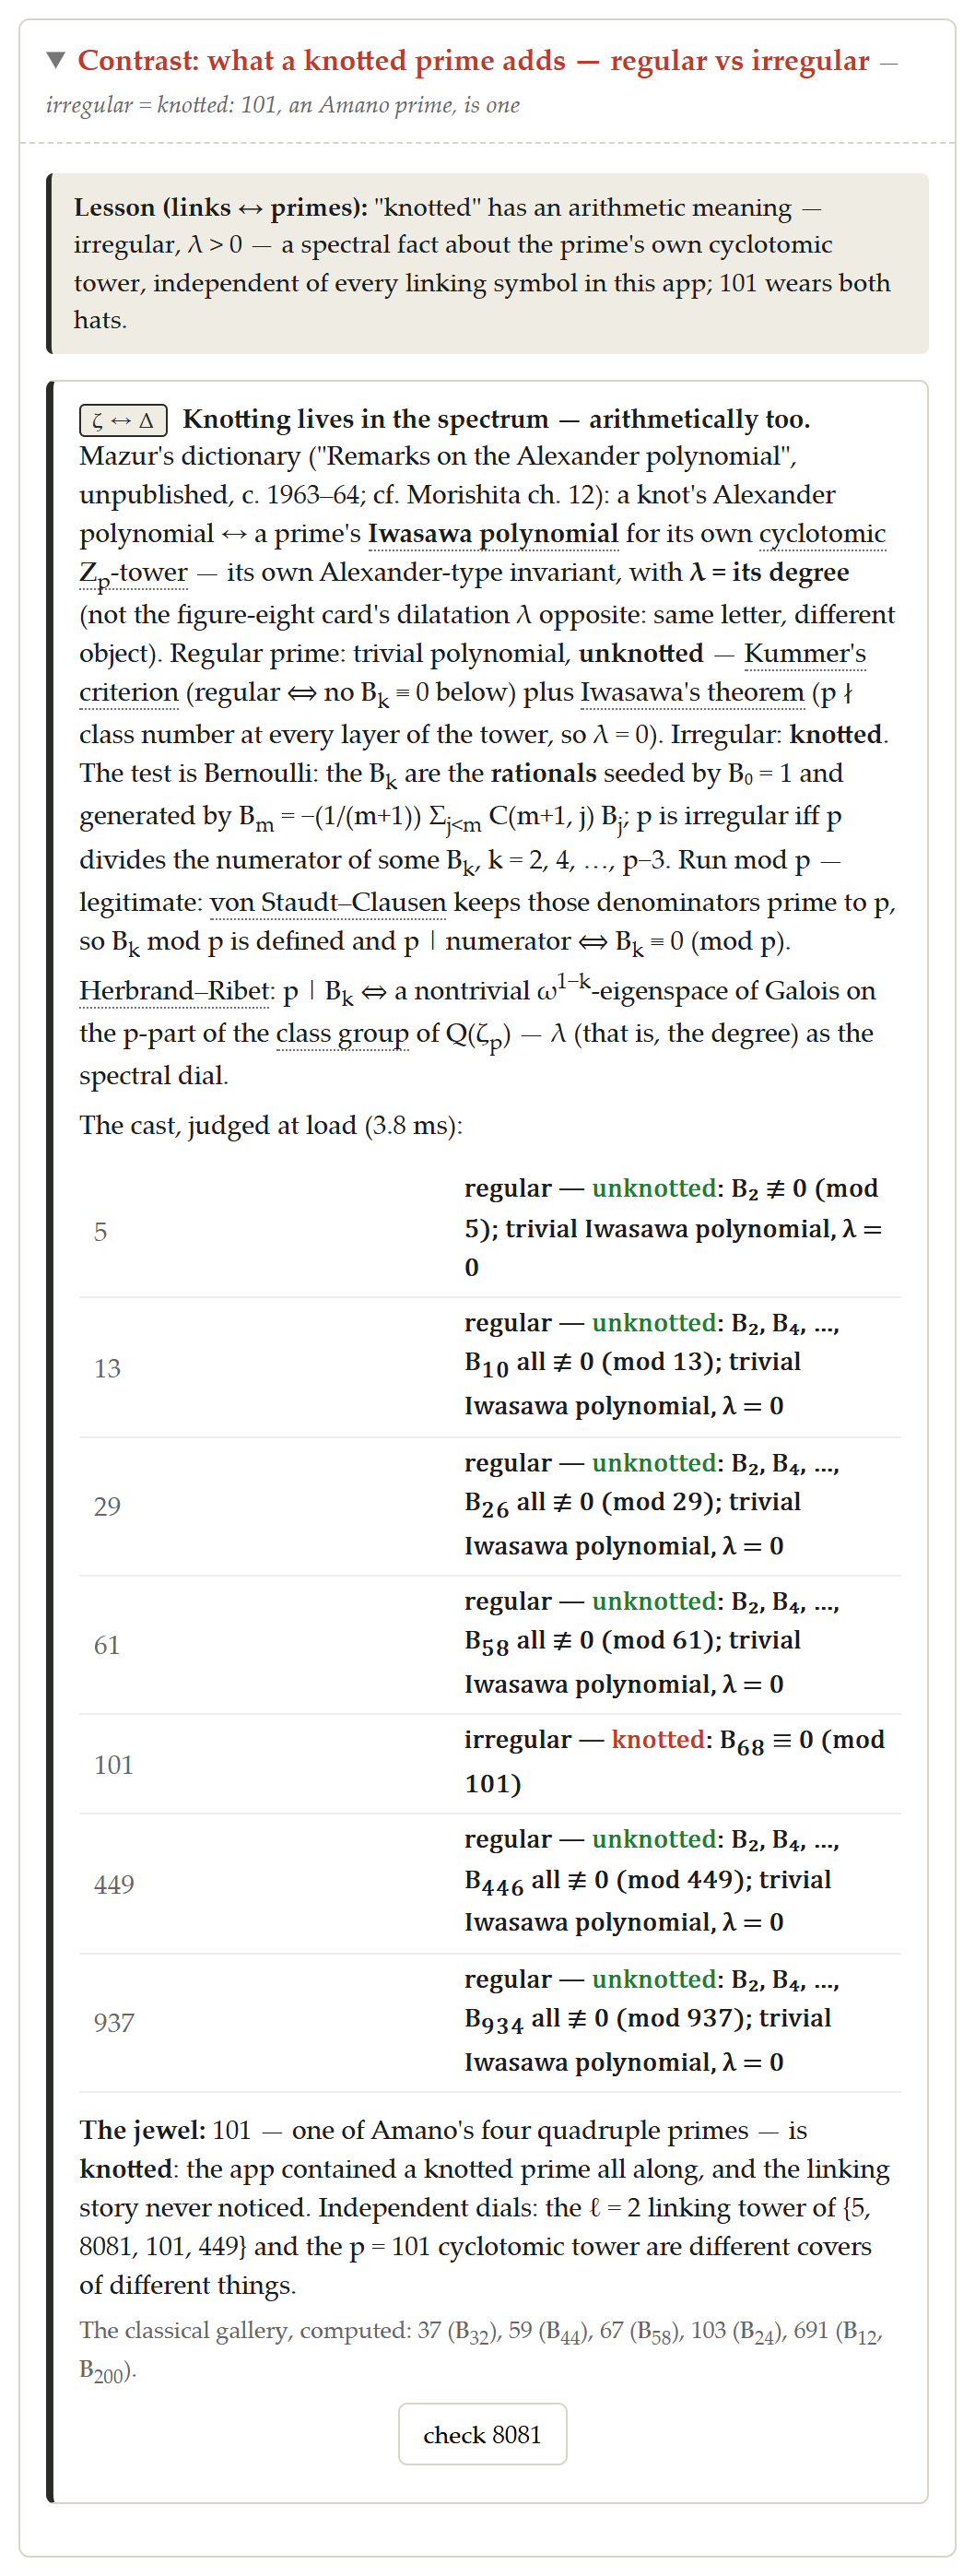
\includegraphics[width=\linewidth,trim=0 0 0 1387,clip]{img/31-knotted-card.png}
\end{columns}
\vspace{2pt}
{\scriptsize\St{Mazur's mirror of knotting: a prime's own cyclotomic tower and its Iwasawa polynomial; regular $=$ unknotted, irregular $=$ knotted. And \textbf{101, one of Amano's own primes, is irregular} ($B_{68}\equiv 0 \pmod{101}$, computed at load). The cast contained a knotted prime all along; the linking story never noticed --- independent dials.}}
\kleinnote{Math: the right kind of surprise --- the dictionary generated a question one column alone would not have asked.}
\end{frame}

% ---------------------------------------------------------------- 24 capstone + ladder
\begin{frame}{Frobenius as a matrix; Chebotarev in plain sight}
\begin{columns}[T]
\column{0.52\textwidth}\shot[0.62\textheight]{img/33-ladder-937.png}
\column{0.46\textwidth}
\shot[0.34\textheight]{img/32-capstone.png}
{\scriptsize\St{Any odd unramified $q$ gets its matrix in $N_3(\mathbb{F}_2)$, live; Chebotarev promises the classes equidistribute (density $1/8$ for the identity, for the corner, \dots) --- the app is the demonstration bench, not the proof, and says so on the Q\&A tab.}}
\end{columns}
\end{frame}

% ---------------------------------------------------------------- 25 QA + breakage
\begin{frame}{The closing move: the failure list}
\begin{columns}[T]
\column{0.52\textwidth}\shot[0.7\textheight]{img/34-qa-first.png}
\column{0.46\textwidth}
\shot[0.44\textheight]{img/35-qa-breakage.png}
{\scriptsize\St{Fourteen of your questions are pre-answered on the Q\&A tab, each answer jumping back into the app. The last one is the five-fracture failure list --- archimedean place, no arithmetic hyperbolic geometry, the $B_4$ model gap, $\mathbb{Z}[t^{\pm1}]$ vs.\ $\Lambda$, not a functor.}}
\medskip
{\scriptsize\K{The failure list is the most convincing slide in the deck. It usually is.}}
\end{columns}
\end{frame}

% ---------------------------------------------------------------- 26 selftests
\begin{frame}{Proof of honesty: the suite, on stage}
\shot[0.7\textheight]{img/36-selftests.png}
{\scriptsize\St{101 checks --- recomputing the numbers and asserting the prose against the rendered page. Run live as the last click of the talk: \textbf{101/101 pass}.}}
\end{frame}

% ---------------------------------------------------------------- 27 notebook math
\begin{frame}{Klein's notebook --- mathematics}
\begin{itemize}\itemsep4pt\footnotesize
\item[A1.] \textbf{Modules on screen.} $\tau\doteq\Delta$ and $f_\Lambda\doteq L_p$ are statements about modules; show one \emph{presentation matrix} per side (Wirtinger/Alexander matrix; its $\Lambda$-analogue). Principal request.
\item[A2.] \textbf{One computed surface picture.} All rung figures are honest schematics; compute $\gamma=\Sigma_1\cap\Sigma_2$ once from the drawn crossings. ``Computed numbers, cartoon geometry'' --- close the gap once, visibly.
\item[A3.] \textbf{Five components as the thesis problem.} Topology ready ($N_5(\mathbb{F}_2)$, order 1024); arithmetic lacks the quintuple independence theorem. Do not soften.
\item[A4.] \textbf{Chebotarev tally.} A running class-count on the Ladder tab against densities $1/8,\dots$ --- quantitative without pretending to prove a density theorem.
\item[A5.] \textbf{Suite hygiene.} The new Q\&A self-test is state-fragile (asserts cards closed at run time); rewrite state-robustly when the freeze lifts.
\end{itemize}
\end{frame}

% ---------------------------------------------------------------- 28 notebook legibility
\begin{frame}{Klein's notebook --- legibility (future presentations)}
\begin{itemize}\itemsep3pt\footnotesize
\item[B1.] \textbf{Trim superfluous framing} (author's directive): e.g.\ the Q\&A intro paragraph compresses to one working sentence. Rule for the pass: every sentence states mathematics, states provenance, or points somewhere --- cut the rest.
\item[B2.] \textbf{Triples side-by-side} (author's directive): strict mirror-rows so each topological cell and its arithmetic twin share a row and height (rung 2's half-empty cell is the exhibit).
\item[B3.] Long-scroll tabs: sticky mini-nav on Triples and Zeta.
\item[B4.] Tooltips don't project: presentation mode --- larger base font, pin-all-in-section.
\item[B5.] Card choreography: URL-hash deep links so each beat is one click.
\item[B6.] Self-tests one keystroke away for the closing beat.
\item[B7.] In-figure label sizes $+25\%$ in presentation mode.
\end{itemize}
\begin{alertblock}{\footnotesize Standing rule}\scriptsize The app is \textbf{frozen}: none of A1--A5, B1--B7 is implemented until these notes are reviewed with the author. Full text: \texttt{presentation-notes.md}.\end{alertblock}
\end{frame}

\begin{frame}{}
\begin{center}
{\large ``Send me the link --- and next time, presentation matrices.''}\\[10pt]
{\footnotesize the app: \texttt{index.html} \quad the dialogue: \texttt{klein-dialogue.md} \quad the notes: \texttt{presentation-notes.md}}
\end{center}
\end{frame}

\end{document}
